\newcommand{\norm}[1]{\left\lVert#1\right\rVert}
\newcommand{\KL}[2]{D_{\mathrm{KL}} \bigl( #1 ~||~ #2 \bigr)}
\newcommand{\trans}{\mathbf{T}}
\newcommand{\qex}{Q_{\text{explore}}}
\newcommand{\qtask}{Q_{\text{task}}}
\newcommand{\tex}{\tau_{\text{explore}}}
\newcommand{\ttask}{\tau_{\text{task}}}
\newcommand{\pitask}{\pi_{\text{task}}}
\newcommand{\piexplore}{\pi_{\text{explore}}}
\newcommand{\algname}{Decoupled Exploration and Exploitation Policies} % name TBD
\newcommand{\algshort}{DEEP} % name TBD

\section{Introduction}
Recent progress in reinforcement learning (RL) for continuous control has led to significant improvements in sample complexity and performance.
While earlier on-policy algorithms required hundreds of millions of environment steps to learn, recent off-policy algorithms have brought the sample complexity of model-free RL in range of solving tasks on real robots \citep{haarnoja2018softapp}.

In parallel, a rich literature has been developed for directed exploration in deep reinforcement learning, inspired in part by the theoretical impact of exploration on sample complexity.
% \citep{Stadie2015IncentivizingEI,Osband2016DeepEV,houthooft2016vime,pathak2017curiosity,Tang2017Exploration,burda2018exploration,Fortunato2018NoisyNF,Plappert2018ParameterSN,osband2019deep,Badia2020NeverGU,Machado2020CountBasedEW,Rashid2020OptimisticEE,Dean2020SeeHE}.
The bulk of these methods fall into the family of bonus-based exploration (BBE) methods, in which a policy receives a bonus for visiting states deemed to be interesting or novel.
BBE algorithms have enabled RL to solve a variety of long-horizon, sparse-reward tasks, most notably the game Montezuma's Revenge from the Arcade Learning Environment (ALE) \citep{Bellemare2015TheAL}.

These two subfields both aim to minimize the sample complexity of model-free RL, and their methods are in principle perfectly complementary.
Off-policy algorithms extract improved policies from data collected by (notionally) arbitrary behavior, and their performance is limited only by the coverage of the data;
meanwhile exploration generates data with improved coverage.
% -- whose performance is limited only by the coverage of the data --
% from data collected by (notionally) arbitrary behavior, while exploration methods generate data with improved coverage.
% Off-policy algorithms extract improved policies from (notionally) arbitrary data, with performance in principle limited only by the coverage of the data, while exploration methods generate data with improved coverage.
However, to date the impact of directed exploration techniques on sample-efficient control has been minimal, with state of the art algorithms using undirected exploration such as maximum-entropy objectives.
In this paper we investigate the missing synergy between off-policy continuous control and directed exploration.


We find that BBE is poorly suited to the few-sample regime due to slowly-decaying bias in the learned policy and slow adaptation to the non-stationary exploration bonus.
Bias due to optimizing a reward function other than the task reward leads a policy trained with BBE to exhibit poor performance until the bonus decays toward zero.
Meanwhile, the non-stationary (continually decreasing) exploration bonus cannot necessarily be optimized by a fixed policy, violating one of the core assumptions of RL.
This leads to slow exploration as the policy adapts only gradually, especially in the off-policy case where replay buffers will contain stale rewards.
These observations underline research by \citet{Taiga2020On} showing that across the ALE, no BBE algorithm outperforms undirected $\varepsilon$-greedy exploration.

We demonstrate that bias and slow coverage are the culprits of BBE's lackluster performance by proposing a new exploration algorithm, \algname{} (\algshort{}), which addresses these limitations.
\algshort{} decouples the learning of a \emph{task policy}, which is trained to maximize the true task reward, and an \emph{exploration policy}, which maximizes only the exploration bonus.
Both policies are trained off-policy using data collected according to the product of the two policy distributions.
Unlike the policy learned by BBE, \algshort{}'s task policy is always unbiased in the sense that it reflects the current belief about the optimal action in each state.
Furthermore, this decoupling allows \algshort{} to aggressively update the exploration policy without affecting the convergence of the task policy, thereby adapting more rapidly to the changing exploration bonus.

We perform experiments using policies based on Q-learning \citep{sutton2018reinforcement,mnih2015human} on toy tasks and soft actor-critic (SAC) \citep{haarnoja2018softapp} on larger-scale tasks from the DeepMind Control Suite \citep{tassa2018deepmind}.
Our results show that on tasks with dense rewards and uniform resets, BBE often performs worse than the underlying policy-learning algorithm while \algshort{} incurs no cost for exploring.
On tasks with more natural resets and sparse rewards, \algshort{} covers the state space more rapidly than BBE and reaches peak performance in a fraction of the samples required with undirected exploration.
In total, \algshort{} strictly outperforms undirected exploration while solving many sparse environments just as fast as dense ones.


\section{Background}

\subsection{Notation}

A Markov decision process (MDP) $\mdp$ consists of a tuple $(\mathcal{S}, \mathcal{A}, P, R, \gamma)$, where $\mathcal{S}$ is the state space, $\mathcal{A}$ is the action space, $P$ is the transition function mapping $\mathcal{S} \times \mathcal{A}$ to distributions on $\mathcal{S}$, $R$ is the scalar reward function on $\mathcal{S} \times \mathcal{A}$, and $\gamma$ is the discount factor.
We use lower-case $(s, a, r)$ to refer to concrete realizations of states, actions, and rewards.
We use $\mdp_f$ to denote the MDP $\mdp$ with the original reward function $R$ replaced by another function $f$.
For convenience we assume exploration rewards are within $[0, 1]$, and we define $\bar{r} = \nicefrac{1}{1 - \gamma}$, which is the maximum discounted value possible.


\subsection{Bonus-based exploration: a recipe for exploration in deep RL} \label{sec:intrinsic_rewards}

Bonus-based exploration has emerged as the standard framework for exploration in the deep reinforcement learning community.
In this framework, an agent learns in a sequence of MDPs $\widetilde{\mdp} = \{\mdp_{\widetilde{R}_n} \}_{n=1}^N$ where the reward function $\widetilde{R}_n$ changes as a function of each transition.
A typical choice is $\widetilde{R}_n = R + R^+_n$, where $R^+_n$ is an exploration bonus which measures the ``novelty'' of a transition $(s, a, s')$ given the history of all transitions up to $n$.
After taking each transition $(s, a, s')$, the reward $\widetilde{r} = \widetilde{R}_n(s, a, s')$ is calculated and the tuple $(s, a, s', \widetilde{r})$ is added to a replay dataset $D$.
The agent optimizes its reward in this (non-stationary) MDP $\widetilde{\mdp}$ via some model-free RL algorithm operating on the replay dataset.
The realization of a particular algorithm in this family amounts to defining a novelty function and picking a model-free RL algorithm \citep{Stadie2015IncentivizingEI,houthooft2016vime,bellemare2016unifying,pathak2017curiosity,Tang2017Exploration,burda2018exploration,Machado2020CountBasedEW}.
We illustrate this recipe in \cref{alg:bbe}.

\paragraph{Pseudo-counts.}
Building upon theoretically-motivated exploration methods for discrete environments \citep{strehl2008analysis}, \citet{bellemare2016unifying} proposed to give exploration bonuses based on a \emph{pseudo-count} function $\hat N$.
A pseudo-count has two key properties.
Like a true count, a pseudo-count increases by 1 each time a state (or state-action pair) is visited.
Unlike a true count, a pseudo-count generalizes across states and actions; that is, when a state $s$ is visited, the pseudo-count for nearby states $s + \varepsilon$ may increase as well.


\begin{figure*}
% \begin{minipage}[b]{\textwidth}
\begin{algorithm}[H]
    % \small
    \centering
    \caption{Bonus-based exploration}\label{alg:bbe}
    \begin{algorithmic}[1] % The number tells where the line numbering should start
        \Require{replay dataset $D$, policy $\pi$, bonus $R^+_n$}
        \item[]
        \State $n \gets 0$
        \Repeat
            \For{one episode}
                \item[]
                \item[]
                \State Collect $(s, a, s', r) \sim P(s, \pi(s))$
                \State $\widetilde{r} \gets r + R^+_n(s, a, s')$
                \State $D \gets D \cup (s, a, s', \widetilde{r})$
                \State $R^+_{n+1} \gets \text{Update}(R^+_n, (s, a, s'))$
                \State $n \gets n + 1$
            \EndFor
            \State Train $\pi$ with samples from $D$
        \Until{$n = N$}
    \end{algorithmic}
\end{algorithm}
% \end{minipage}
\hfill

% \begin{minipage}[b]{\textwidth}
\begin{algorithm}[H]
    % \small
    \centering
    \caption{\algname{}}\label{alg:deep}
    \begin{algorithmic}[1]
        \Require{replay dataset $D$, temperature $\tau$,}
        task policy $\pitask$, exploration policy $\piexplore$, bonus $R^+_n$
        % \Require{policy $\pi$, exploration value $\qex$}
        \State $n \gets 0$
        \Repeat
        \For{one episode}
            \State Update $\piexplore$ on $\mdp_{R^+_n}$
                \State Set $\beta(a|s) \propto \pitask(a|s) \cdot \piexplore(a|s)$ %by \cref{eq:behavior_policy}
                \State Collect $(s, a, s', r) \sim P(s, \beta(s))$
                \item[]
                \State $D \gets D \cup (s, a, s', r)$
                \State $R^+_{n+1} \gets \text{Update}(R^+_n, (s, a, s'))$
                \State $n \gets n + 1$
            \EndFor
            \State Train $\pitask$ with samples from $D$
        \Until{$n = N$}
    \end{algorithmic}
\end{algorithm}
% \end{minipage}
\caption{
Comparison of classic bonus-based exploration (BBE) with our method (\algshort{}).
BBE computes exploration bonuses at the time of visiting a transition, adds them to the real rewards, and uses a replay buffer of experience to learn a policy.
\algshort{} separates the exploration policy $\piexplore$ from the task policy $\pitask$, allowing $\pitask$ to be an unbiased estimate of the optimal policy throughout training.
It always uses the \emph{current} exploration reward function $R_n^+$ when updating the exploration value function, and is fast-adapting to deal with the non-stationary bonus MDP.
% \red{(include the reward function as an input and show it updating)}
% Finally \algshort{}'s behavior policy actions and updates are optimistic, ensuring the agent will reach and take transitions it has never seen.
}
\end{figure*}


\section{Limitations of bonus-based exploration}

\begin{figure}[h]
    \centering
    \begin{subfigure}[b]{0.49\textwidth}
        \centering
        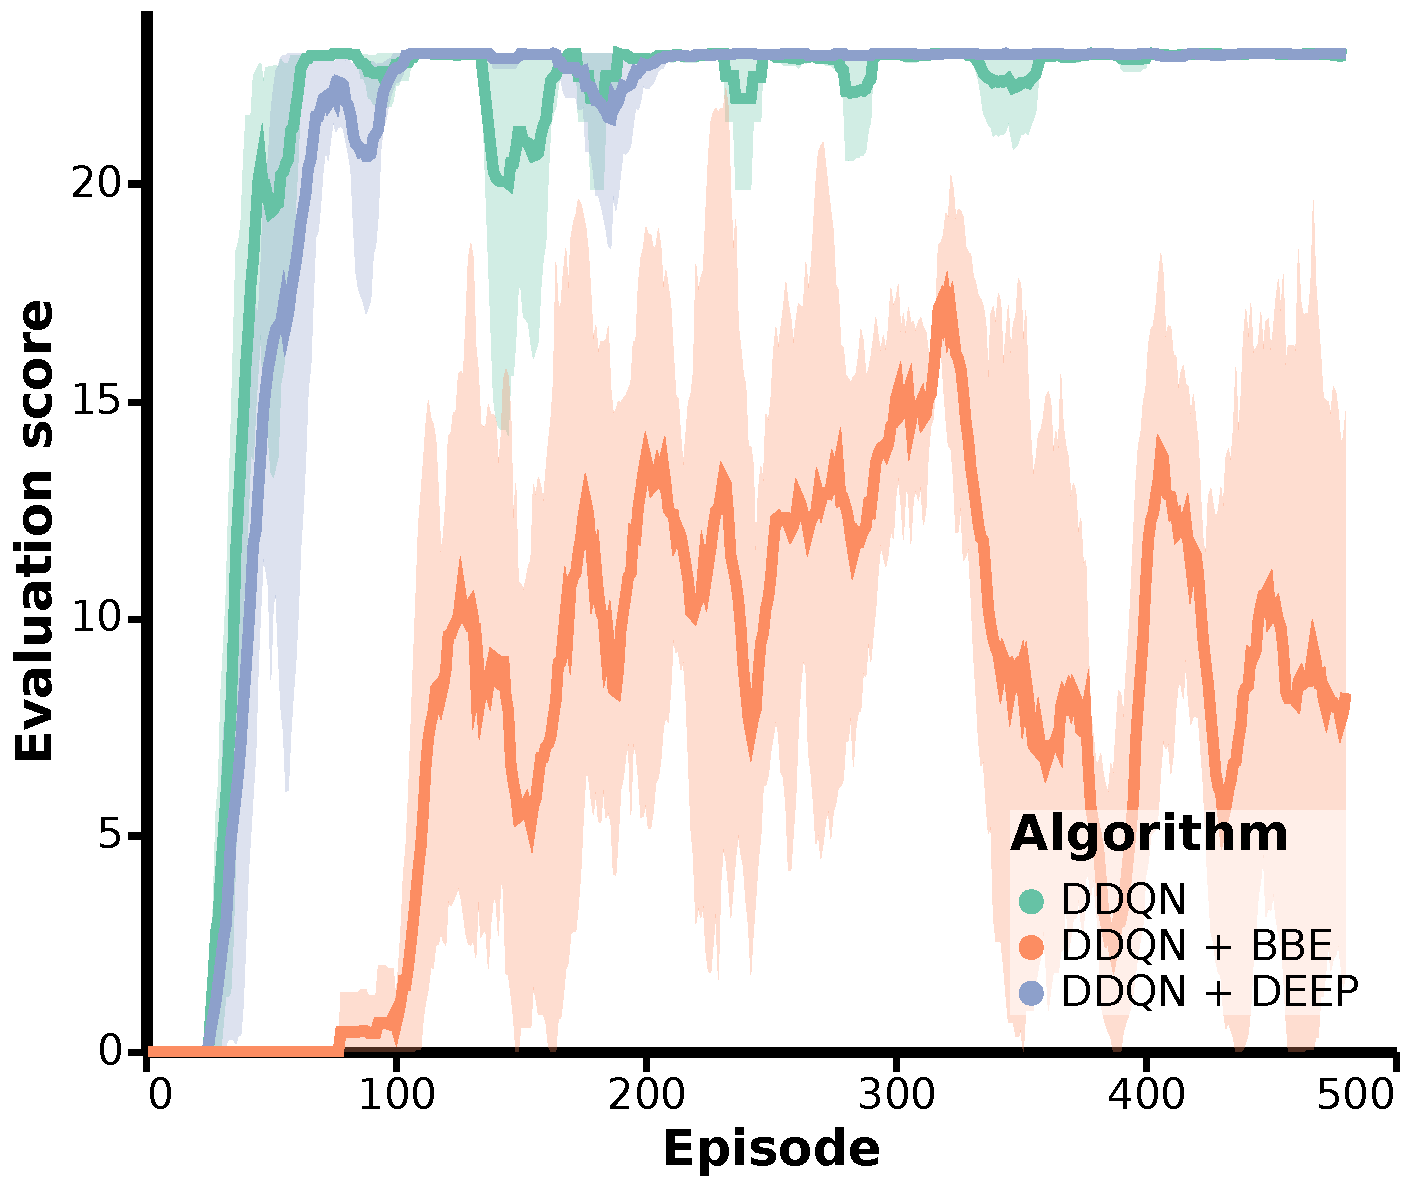
\includegraphics[width=0.8\textwidth]{figures/deep/grid40_warmstart.pdf}
        \caption{Reward}
    \end{subfigure}
    \hfill
    \begin{subfigure}[b]{0.49\textwidth}
        \centering
        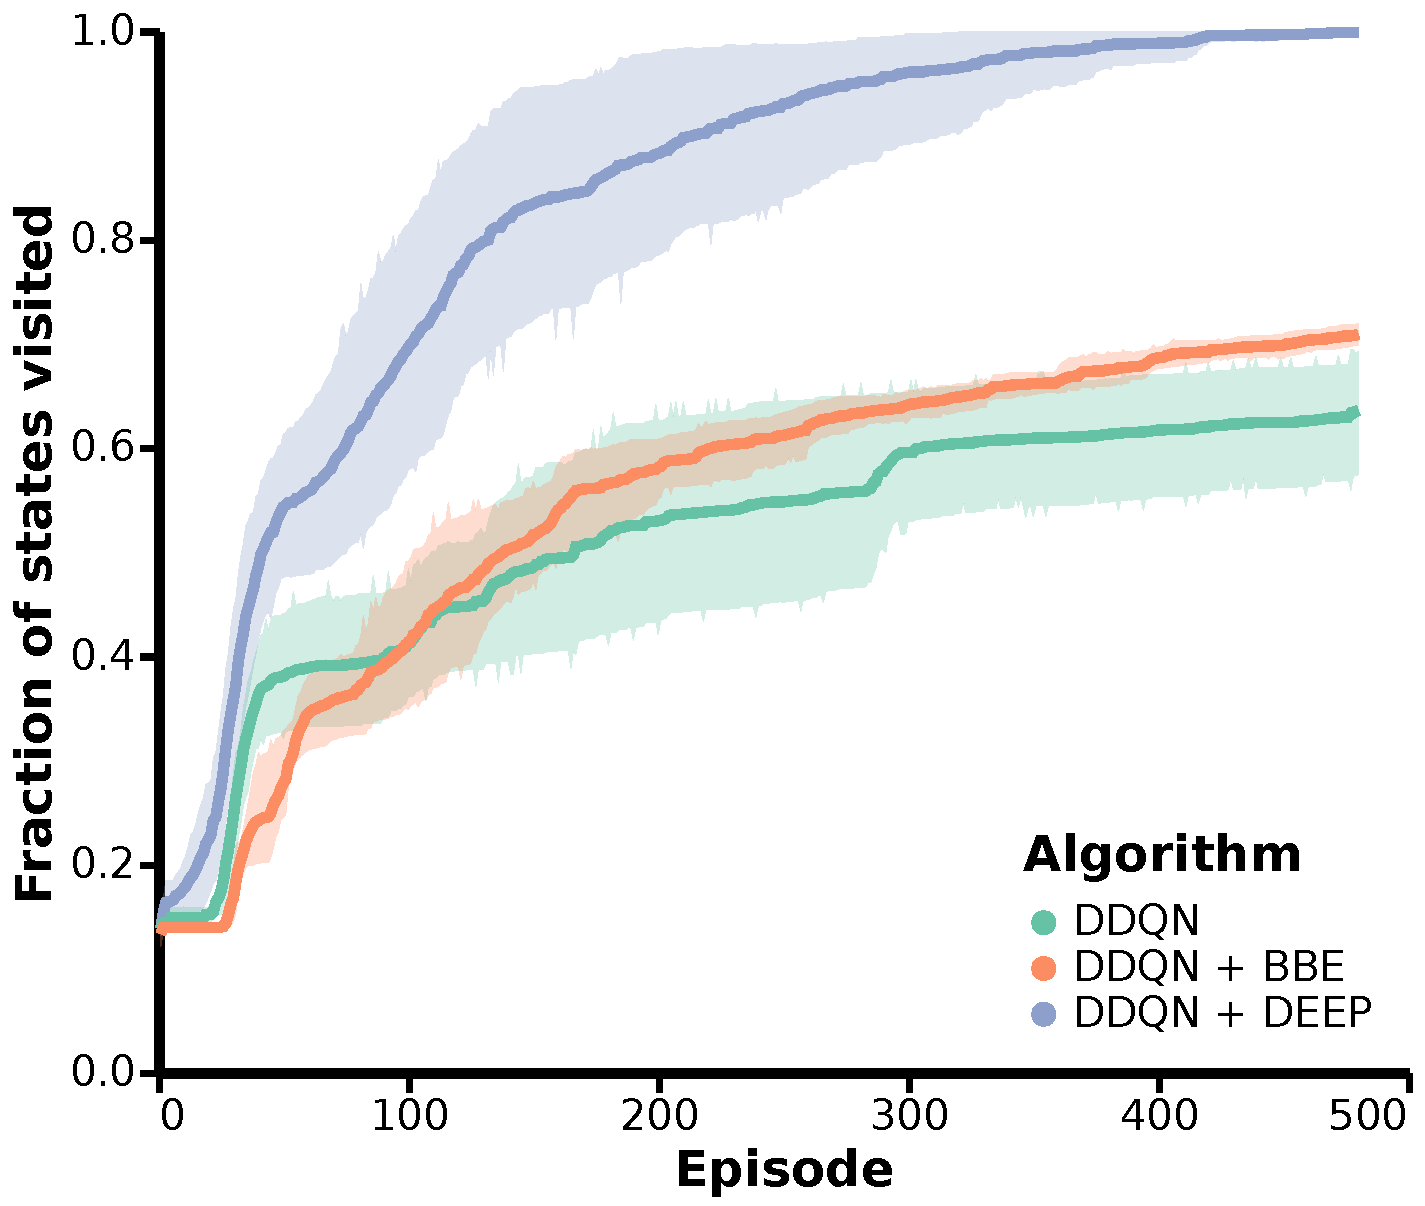
\includegraphics[width=0.8\textwidth]{figures/deep/grid40_warmstart_visits.pdf}
        \caption{Coverage}
    \end{subfigure}
    \caption{Experiments in a $40 \times 40$ grid-world environment with one goal state, where learning algorithms were warm-started with 20 episodes of data from a skilled policy.
    \textbf{(a)} With enough signal to find the goal, DDQN (Double DQN, \citet{Hasselt2016DeepRL}) alone rapidly converges to the optimal policy. BBE introduces bias, causing the policy to continually explore. Our method, \algshort{}, learns the task policy just as rapidly as DDQN alone.
    \textbf{(b)} Though it performs well, DDQN simply goes to the goal during each train episode and does not explore other options. BBE continues to seek out new states at a slow but steady rate. \algshort{} explores far more than BBE during data collection despite simultaneously performing just as well as DDQN at evaluation time.}
    \label{fig:gridworld_warmstart}
\end{figure}

The bonus-based exploration algorithm, illustrated in \Cref{alg:bbe}, has two weaknesses which limit its usefulness for sample-efficient policy learning.


\paragraph{Bias with finite samples.}
Because they estimate the optimal policy on the modified MDP $\mdp'$, bonus-based exploration algorithms learn biased policies as long as the exploration bonus is nonzero.
According to theory, the exploration bonus should be scaled larger than is done in practice \citep{strehl2008analysis} and decay slower than $\nicefrac{1}{N(s)}$ \citep{Kolter2009NearBayesianEI} in order to guarantee convergence to the optimal policy.
This behavior, shown in \Cref{fig:gridworld_warmstart}, can result in slow convergence to the optimal policy and substantially biased policies after a practically feasible number of samples.

\begin{figure}[h]
    \begin{center}
        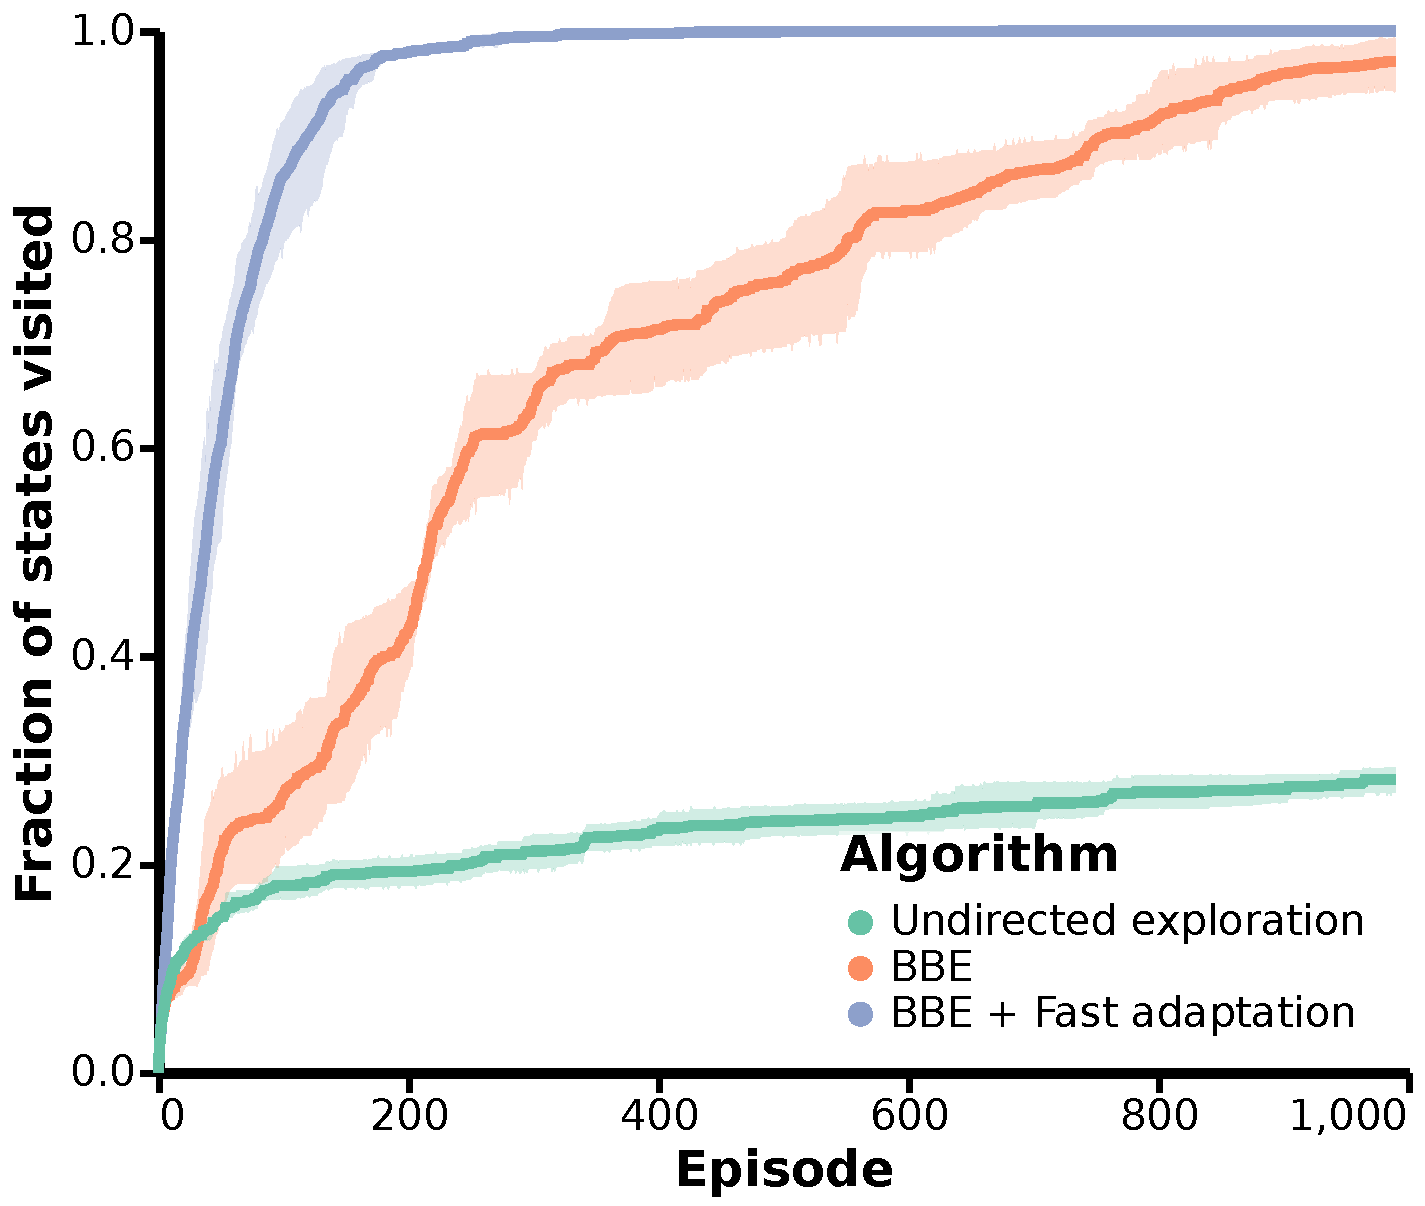
\includegraphics[width=0.35\textwidth]{figures/deep/grid40_visits_neurips.pdf}
    \end{center}
    % \caption{A test of pure exploration speed. Undirected exploration with a uniformly random policy covers the state space very slowly. BBE, with its ability to seek unknown states, is faster. However, BBE does not adapt rapidly to the changing rewards, leading it to be slower than the fast adaptation scheme we propose.}
    \caption{Pure exploration}
    \label{fig:gridworld_visits}
\end{figure}

% \caption{Two experiments in a $40 \times 40$ grid-world environment with one goal state. \textbf{(a)} Learning algorithms warm-started with 20 episodes of data from a skilled policy. Since there is plenty of signal to find the goal, DDQN without exploration rapidly converges to the optimal policy. BBE introduces bias, causing the policy to continually explore. Our method, \algshort{}, learns the task policy just as rapidly as DDQN alone.
% \textbf{(b)} A test of pure exploration speed. Undirected exploration with a uniformly random policy covers the state space very slowly. BBE, with its ability to seek unknown states, is faster. However, BBE does not adapt rapidly to the changing rewards, leading it to be slower than the fast adaptation scheme we propose.\textcolor{red}{TOBI: TODO these need to take the count function/bonus reward as input and update them.}}


\paragraph{Slow adaptation to changing rewards.}
Algorithms in this family update the policy according to the schedule of the underlying model-free RL algorithm -- for example at the end of each episode.
This works well for the stationary MDPs that these algorithms were developed for, but the modified MDP $\mdp'$ which represents the exploration problem is non-stationary.
This leads to an agent which determines the most novel state and then stays there for an entire episode.
This degenerate behavior leads to potentially exploring only a single state per episode instead of visiting a sequence of new states as the reward function evolves.\endnote{Some implementations of bonus-based exploration may update the policy within an episode, for example via a single gradient step per environment step on transitions sampled i.i.d.~from a replay.
However, such a small update is typically not enough to change the qualitative behavior of the agent and adapting to the changing MDP has not been an emphasis in prior work.}
The use of replay buffers compounds this effect, since algorithms in this family compute exploration rewards at the time the transition is collected, rather than when it is used.
An algorithm which is unaware of the non-stationary nature of the MDP will maximize the return on this mixture of reward functions rather than the reward that incorporates the current bonus, resulting in slow coverage of the environment.
\Cref{fig:gridworld_visits} shows uniform random actions, BBE, and BBE with the fast adaptation scheme we propose in \Cref{sec:fast_adaptation} all exploring in a $40 \times 40$ grid-world without rewards.
While BBE covers the state space much faster than undirected exploration, it is unnecessarily slow.
See Appendix \ref{sec:gridworld-vis} for visualizations.


\section{Decoupled exploration for sample-efficient control}
In this section, we describe a new algorithm called \algname{} (\algshort{}) which addresses the limitations of BBE.
The core insight is that by leveraging off-policy RL algorithms, \algshort{} can learn two policies from the same replay: a task policy $\pitask$, which maximizes the reward on the original MDP $\mdp_R$, and an exploration policy $\piexplore$, which maximizes only the reward on the bonus MDP $\mdp_{R^+_n}$.
This decoupling serves two purposes.
First, it enables good performance even before exploration is complete by using $\pitask$ at test time.
Second, it allows $\piexplore$ to be updated aggressively in order to more closely match the non-stationary bonus MDP; unlike $\pitask$, it is not important that $\piexplore$ converge exactly to an optimal policy.

Like BBE, \algshort{} is a family of algorithms related by their structure; a particular algorithm in this family consists of a choice of an exploration reward function and an off-policy RL algorithm for learning each policy.
Throughout this work, we use a pseudo-count based exploration reward.
For discrete tasks we use Double DQN (DDQN, \citet{Hasselt2016DeepRL}) and Boltzmann policies.
For tasks with continuous actions we use soft actor-critic (SAC) for $\pitask$ and a DDQN policy for $\piexplore$.


\subsection{Pseudo-count estimation} \label{sec:kernel_counts}
Following \citet{bellemare2016unifying}, we use an exploration reward derived from pseudo-counts.
Instead of the high-dimensional pixel observations of the ALE, Control Suite has low-dimensional ($<$100-D) observations corresponding to joint and object locations and velocities.
% This allows us to replace the pseudo-counts extracted from a density estimator used in that work with a directly specified pseudo-count function based on kernels.
This lower dimensionality renders extracting pseudo-counts from a density estimator unnecessary, and in our experiments we specify a pseudo-count function based on kernels.
For a real-valued state-action pair $x = [s, a]$ and a set of previous observations $\{x_i\}_{i=1}^n$, define the pseudo-count of $x$ and the exploration reward as
\begin{align}
    \hat N_n(x) = \sum_{i=1}^n k(x_i, x) && R^+_n(s, a) = \hat N_n \big([s, a] \big)^{-1/2}
\end{align}
where $k$ is a kernel function scaled to have a global maximum $k(x, x) = 1$.
This satisfies the key requirement for a pseudo-count function, namely that a visit to a state $x$ increases $\hat N(x)$ by 1 and $\hat N(x')$ by at most 1 for any other state $x'$.
In our experiments we use a Gaussian kernel (scaled to have a maximum value of 1) with diagonal covariance.
For implementation details see Appendix \ref{sec:count_implementation}.
% \todo{write the actual reward function}

\subsection{Separating task and exploration policies}

\algshort{} uses two separate policies.
Each is trained off-policy using transitions sampled from the replay buffer; $\pitask$ is updated using the rewards from $R$ logged in the replay, while $\piexplore$ is updated using rewards from $R^+_n$.
Since $\pitask$ is trained only on the rewards for the true task, it is unbiased in the sense that it reflects the current best estimate of the optimal policy.
This stands in contrast to BBE policies, which optimize the sum of task and exploration rewards and thus represent a biased estimate of the optimal task policy until the exploration rewards go to zero.
Our method is agnostic to the choice of algorithm and policy parameterization.
However, it will be most effective with policy learning algorithms that work well when trained far off-policy and produce high-entropy policies (e.g. policies which cover all optimal actions).
For these reasons we use the state-of-the-art maximum-entropy algorithm SAC to learn $\pitask$ in environments with continuous actions. For experiments with discrete action spaces we forego explicitly learning the task policy $\pitask$; instead we learn the task Q-function via DDQN \citep{Hasselt2016DeepRL} and define the task policy as $\pitask(a | s; Q) \propto \exp(Q(s, a) / \tau)$, where $\tau > 0$ becomes a hyperparameter -- we refer to the supplementary material for details.


\subsection{Fast-adapting exploration policy} \label{sec:fast_adaptation}
The non-stationary nature of the exploration reward function poses a challenge to typical model-free RL algorithms, which assume a fixed reward function.
BBE methods update a single policy using a replay buffer which, at a step $n$, contains rewards from a mixture of bonus reward functions $\{R_1^+, \ldots, R_n^+\}$, computed using different past novelty or count estimates.\endnote{See e.g. the code from \citet{Machado2020CountBasedEW}:  \url{https://github.com/mcmachado/count_based_exploration_sr/blob/master/function_approximation/exp_eig_sr/train.py\#L204}}
This results in slow adaptation to the non-stationary objective of exploration.
\algshort{} makes two changes to mitigate the impact of the non-stationarity in the exploration reward function.

First, \algshort{} leverages access to $R^+_n$ to compute exploration rewards when they are needed to update $\piexplore$ rather than when the transition is collected.
We choose to use Q-learning rather than a more sophisticated algorithm in order to learn $\piexplore$ as rapidly as possible; with changing rewards, using a policy to amortize the maximization of a value function as in SAC or DDPG would slow down learning.
We represent $\piexplore$ directly as a Boltzmann policy of this exploration Q-function $\qex$:
\begin{align}
    \piexplore(a \mid s) \propto \exp \left\{ \frac{\qex(s, a)}{\tex} \right\},
\end{align}
where $\tex$ is a temperature hyperparameter.

Second, by decoupling $\piexplore$ from $\pitask$, \algshort{} unlocks the ability to update $\piexplore$ more aggressively without affecting $\pitask$'s convergence to the optimal policy.
This enables the exploration policy to more rapidly adapt to the non-stationary exploration reward.
In our experiments we achieve this by using a larger learning rate and more updates per environment step than is usually done; future work might investigate more sophisticated schemes such as prioritized sweeping \citep{Moore1993PrioritizedSR} or prioritized experience replay \citep{Schaul2016PrioritizedER}.
To improve stability we use DDQN updates and clip Q targets at $\bar{r}$, the maximum discounted exploration value.
% \todo{discuss clipping targets at 100?}

\paragraph{Optimism.} \label{sec:optimistic}
Further adapting $\piexplore$ to the unique properties of the exploration reward function, we propose to leverage optimism in its updates and actions.
We propose to make $\qex$ optimistic by leveraging the pseudo-count function in a manner similar to that proposed by \citet{Rashid2020OptimisticEE}.
We assume that the value function is trustworthy for transitions with very large counts, and very untrustworthy for transitions with near-zero counts.
When the count is zero we impose an optimistic prior which assumes the transition will lead to a whole episode of novel transitions; as the count increases we interpolate between this prior and the learned value function using a weighting function:
\begin{align} \label{eq:optimism}
\qex^+(s, a) = w(s, a) \cdot \qex(s, a) + (1 - w(s, a))  \cdot \bar{r}, \qquad w(s, a) = \frac{\sqrt{N(s, a)}}{\sqrt{N(s, a) + c}}
\end{align}
where $\bar{r} = \nicefrac{1}{1-\gamma}$, is the maximum discounted return in the bonus MDP and $c$ is a small constant representing how many counts' worth of confidence to ascribe to the optimistic prior.
We use this optimistic $\qex^+$ for computing targets for Bellman updates and for computing $\piexplore$ (Eq. \ref{eq:behavior_policy}).
For details of the implementation of the fast-adapting $\piexplore$, see Appendix \ref{sec:fast_updates_appendix}.


\subsection{Product distribution behavior policy}
A good behavior policy should attempt to explore all of the transitions which are relevant for learning the optimal policy.
This entails a trade-off between taking actions which are more novel and ones which are more likely to be relevant to a high-performing policy.
\algshort{} encodes this by representing the behavior policy as a product of the task policy $\pitask$ and the pure-exploration policy $\piexplore$:
\begin{align} \label{eq:behavior_policy}
\beta(a \mid s) \propto \pitask(a \mid s) ~ \piexplore(a \mid s).
\end{align}
% where $\tex$ is a temperature hyperparameter controlling the aggressiveness of the exploration and $\qex^+$ is an optimistic version of the exploration value function (see \Cref{sec:optimistic}).

The choice to parameterize $\beta$ as a factored policy was made for its simplicity and ease of off-policy learning.
Alternative formulations for making this trade-off while preserving the unbiased task policy are possible, and we view the form of our proposed behavior policy as just one option among many.
One alternative would be interleaving the behavior of multiple policies within one episode, akin to e.g. Scheduled Auxiliary Control \citep{Riedmiller2018LearningBP}.

In order to approximately sample from this behavior policy, we use self-normalized importance sampling with $\pitask$ as the proposal distribution:
\begin{enumerate}
    \item Draw $k$ samples $a_1, \ldots, a_k$ from $\pitask$
    \item Evaluate $\piexplore(a_i \mid s)$ for each $i \in 1 \ldots k$
    \item Draw a sample from the discrete distribution $p(a_i) = \piexplore(a_i \mid s) / \sum_{i'} \piexplore(a_{i'} \mid s)$.
\end{enumerate}
Note that since the proposal distribution is $\pitask$, the $\pitask$ terms in computing weights cancel and only the $\piexplore$ terms remain.
Importance weighting is consistent in the limit of $k \to \infty$ but introduces bias towards $\pitask$ \citep{Vehtari2015ParetoSI}.
With small $k$, this bias makes it unlikely that $\beta$ will select actions that are very unlikely under $\pitask$; roughly speaking, this procedure selects the ``most exploratory'' action in the support of the task policy.
This may act as a backstop to prevent the behavior from going too far outside the task policy to be useful.
\algshort{} works best when $\pitask$ is trained in a way that preserves variance in the policy (e.g. SAC's target entropy), enabling the behavior policy to select exploratory actions. In discrete action spaces we additionally use self-normalized importance sampling -- using a uniform proposal over actions -- to obtain samples from $\pitask$ in step 1.
% and \algshort{} with a deterministic task policy would .

% If the RL algorithm for learning $\pitask$
% If the RL algorithm for learning $\pitask$
% As mentioned above, this procedure works best when $\pitask$ is trained in a way that preserves variance in the policy (e.g. by enforcing a minimum entropy in the policy).
% If the choice of RL algorithm does not give such a guarantee importance sampling based on a mix of a random proposal and the task policy could be performed.


\section{Experiments}
% \red{Goals: (1) show that BBE hurts on dense environments, and ours doesn't; (2) show that ours learns fastest on spare environments}

In this section we perform experiments to give insight into the behavior of undirected exploration, BBE, and \algshort{}.
% In particular, we investigate how each algorithm's performance changes as the task requires more exploration
First we perform a set of investigative experiments to probe how \algshort{} interacts with environments with different reward structures.
Then we perform experiments on pairs of benchmark continuous control tasks with easy and hard exploration requirements.

\begin{figure}[h]
    \centering
    \begin{subfigure}[b]{0.49\textwidth}
        \centering
        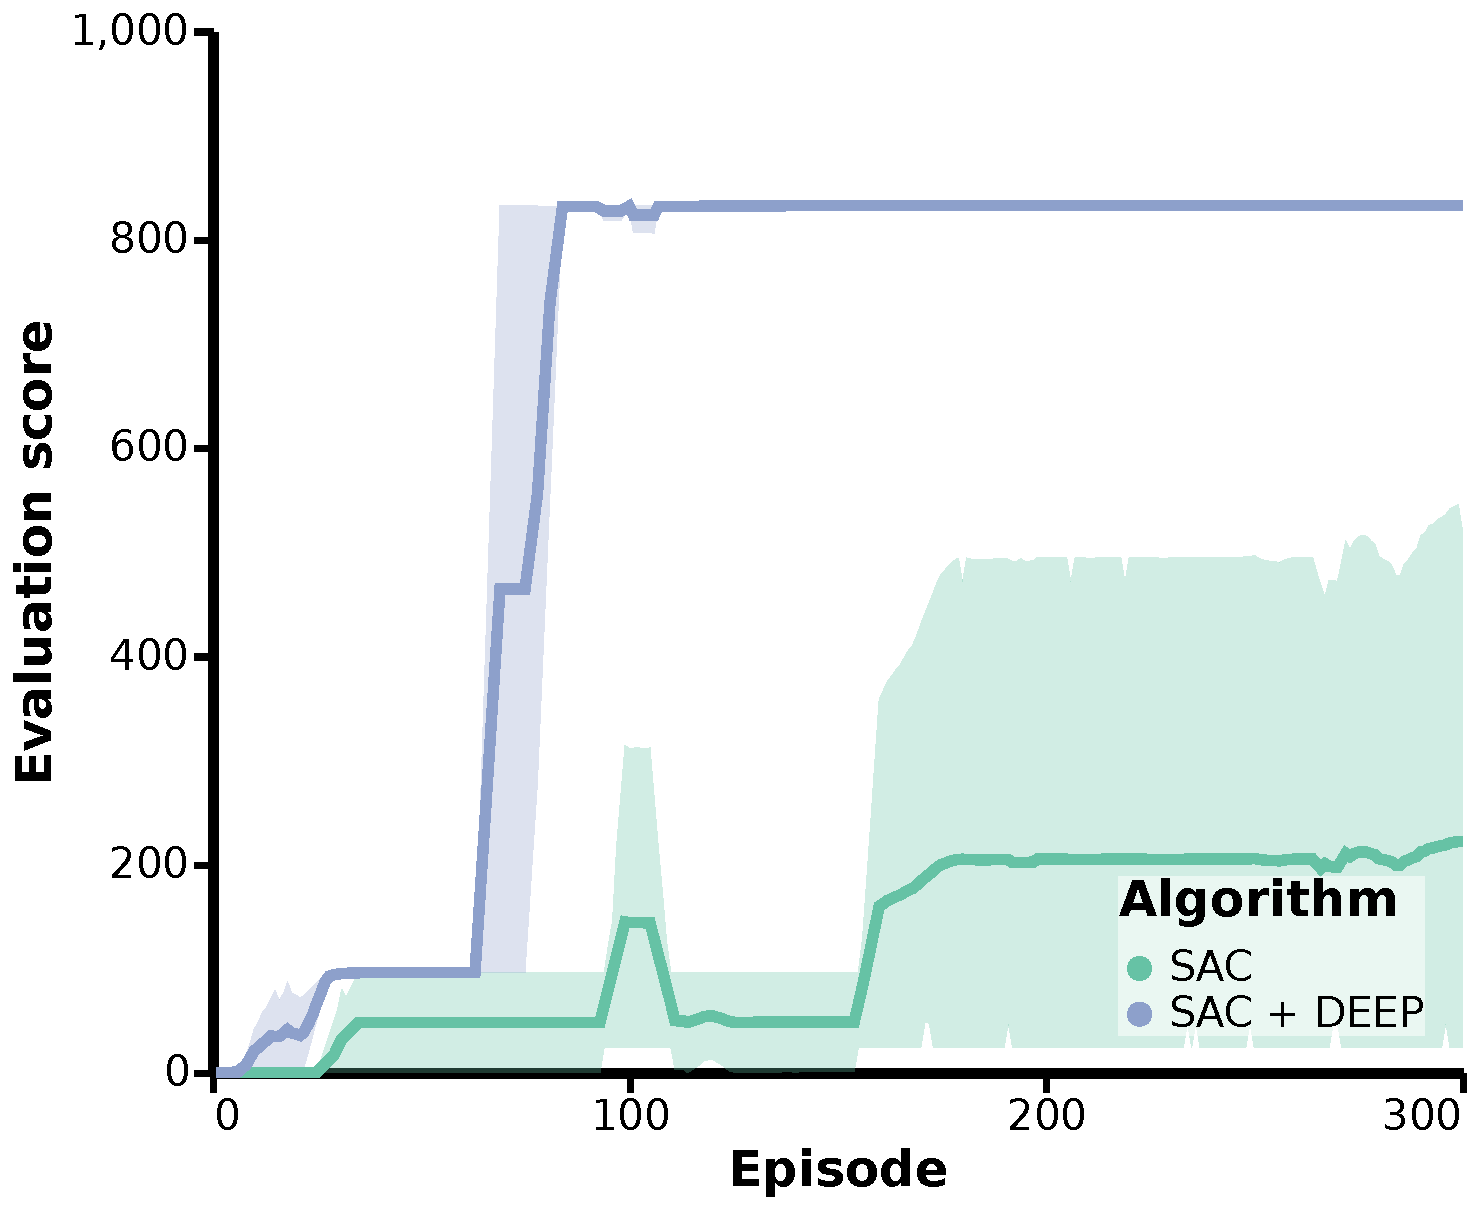
\includegraphics[width=0.8\textwidth]{figures/deep/hallway_velocity_4_distractor.pdf}
        \caption{Local optimum environment} \label{fig:hallway_local_optimum}
    \end{subfigure}
    \hfill
    \begin{subfigure}[b]{0.49\textwidth}
        \centering
        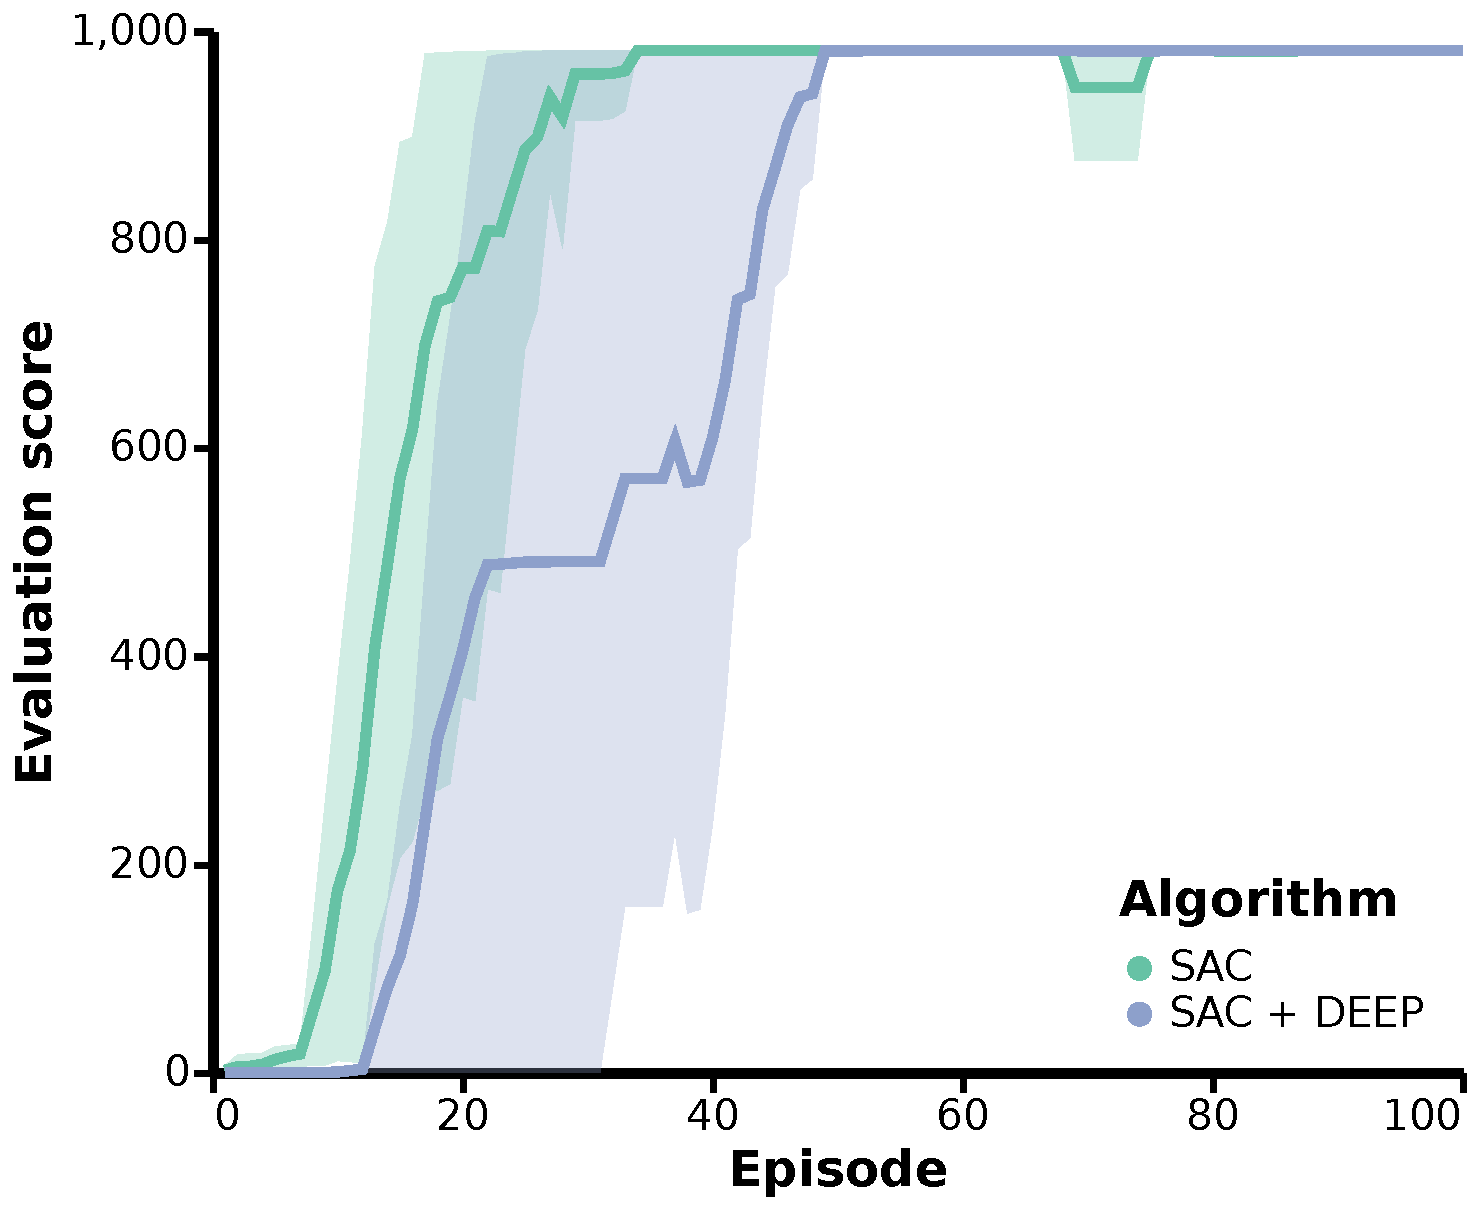
\includegraphics[width=0.8\textwidth]{figures/deep/hallway_velocity_4_inverse_distractor.pdf}
        \caption{Adversarial environment}\label{fig:inverse_distractor}
    \end{subfigure}
    \caption{Two environments illustrating different reward structures.
    \textbf{(a)} An environment with a locally-optimal goal (reward 0.1) near the start state. SAC finds this nearby goal, but doesn't explore far enough to find the real goal (reward 1.0). When trained with \algshort{}, it finds the distractor goal but moves on to the real goal.
    \textbf{(b)} An adversarial environment for \algshort{} which has a very small goal state close to the start state, making it easy to find with random actions but hard with directed exploration.}
    \label{fig:hallway}
\end{figure}

\subsection{Investigative experiments}

We construct a simple MuJoCo \citep{todorov2012mujoco} environment called Hallway to look more closely at how exploration interacts with reward structure.
This environment consists of a long narrow 2D room with the agent controlling the velocity of a small sphere, which starts each episode at one end of this hallway.
The following two experiments share dynamics and differ only in their rewards.

\paragraph{Local optima.}
A valuable role for exploration is enabling an agent to escape from locally optimal behavior.
% behavior that is locally but not globally optimal.
To test this, we add two goal states with shaped rewards to the Hallway environment.
The first is close to the start state but only provides reward at most 0.1, while the second is at the far end of the hallway but provides reward 1.0.
\Cref{fig:hallway_local_optimum} shows that exploration using \algshort{} allows the agent to quickly find its way to the faraway optimal reward while SAC gets stuck in the local optimum.


\paragraph{Limitations.}
% While \algshort{} outperforms SAC in each of the Control Suite environments, there is no such thing as a universally optimal exploration strategy.
\algshort{} covers states quickly, but there is no such thing as a universally optimal exploration strategy.
For example, there exist environments for which the random walk dynamics of undirected exploration find the optimal strategy faster than uniform state coverage.
\Cref{fig:inverse_distractor} provides one such example: a Hallway environment with a very small goal state close to the start state.
SAC discovers this goal faster than SAC + \algshort{}, though \algshort{} does eventually find it as well.


\subsection{Benchmark experiments}
Next we provide experiments based on DeepMind Control Suite \citep{tassa2018deepmind}, a standard benchmark for continuous control RL algorithms.
We introduce versions of several environments which are modified to remove the accommodations that make them solvable without exploration, then provide results of SAC, SAC + BBE, and SAC + \algshort{} on the original and modified environments.

\subsubsection{Results}
\begin{figure}[ht]
    \centering
    \begin{subfigure}[b]{0.24\textwidth}
        \centering
        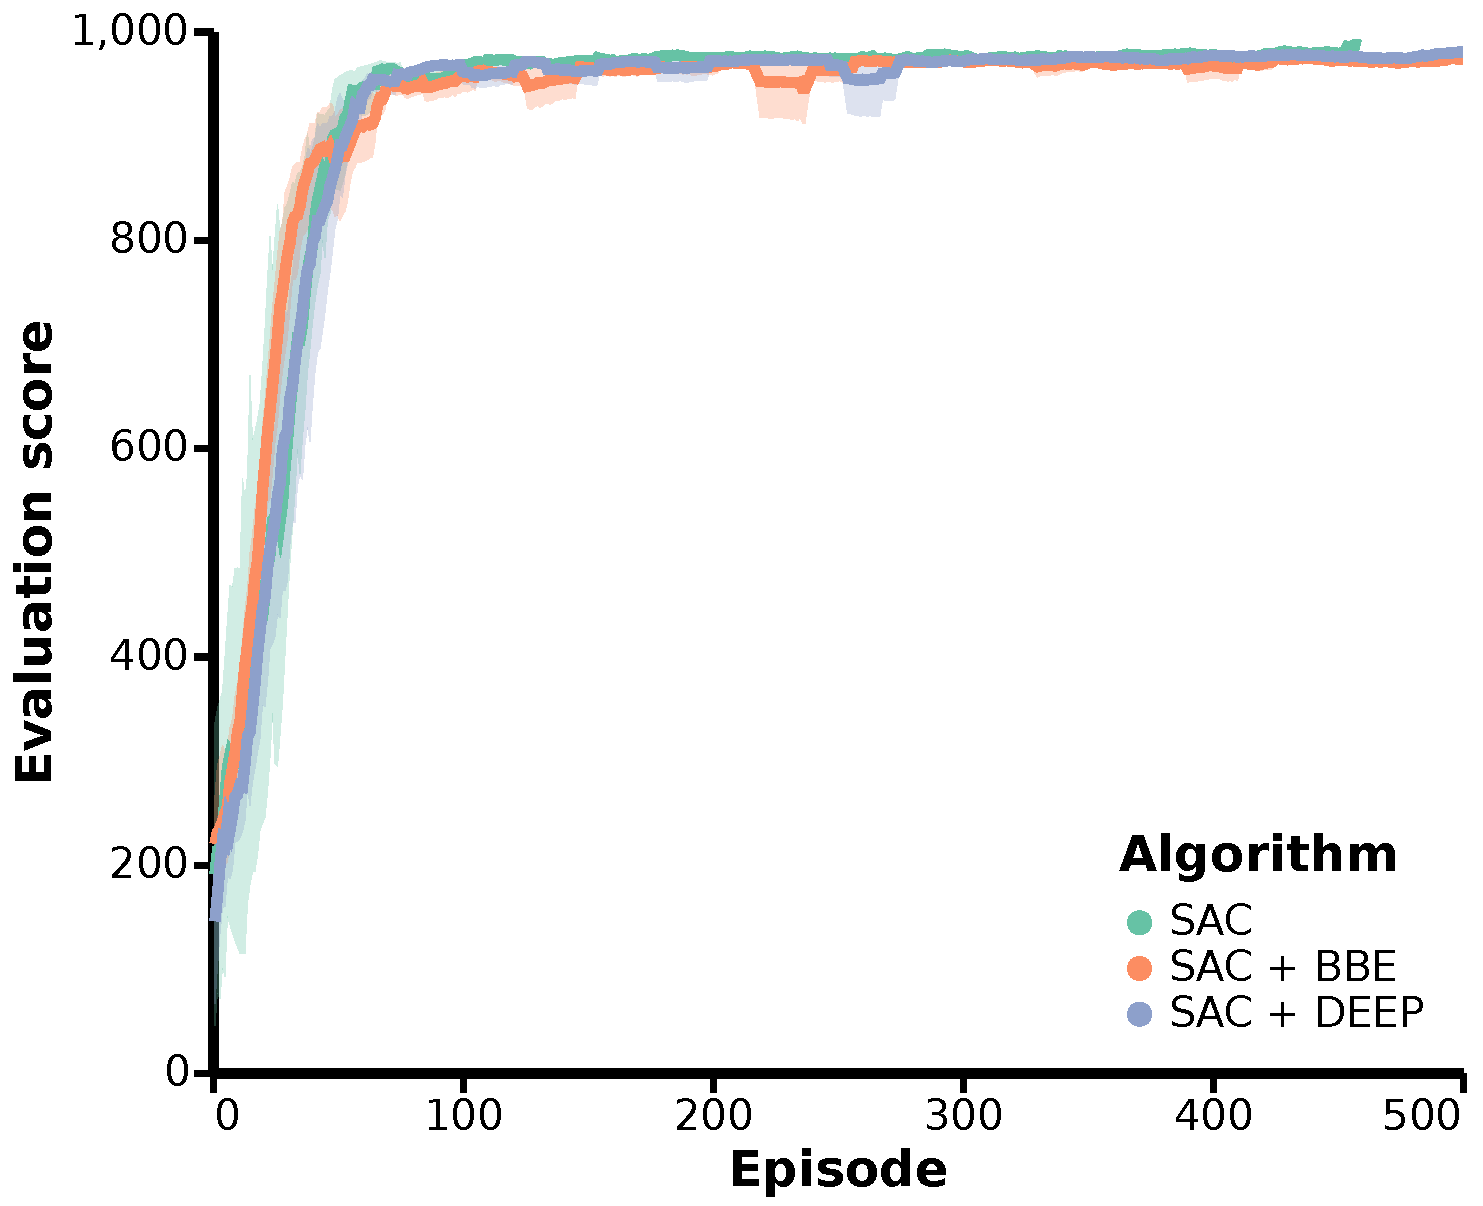
\includegraphics[width=\textwidth]{figures/deep/neurips_ball_in_cup.pdf}
        \caption{Ball-in-cup}
    \end{subfigure}
    \begin{subfigure}[b]{0.24\textwidth}
        \centering
        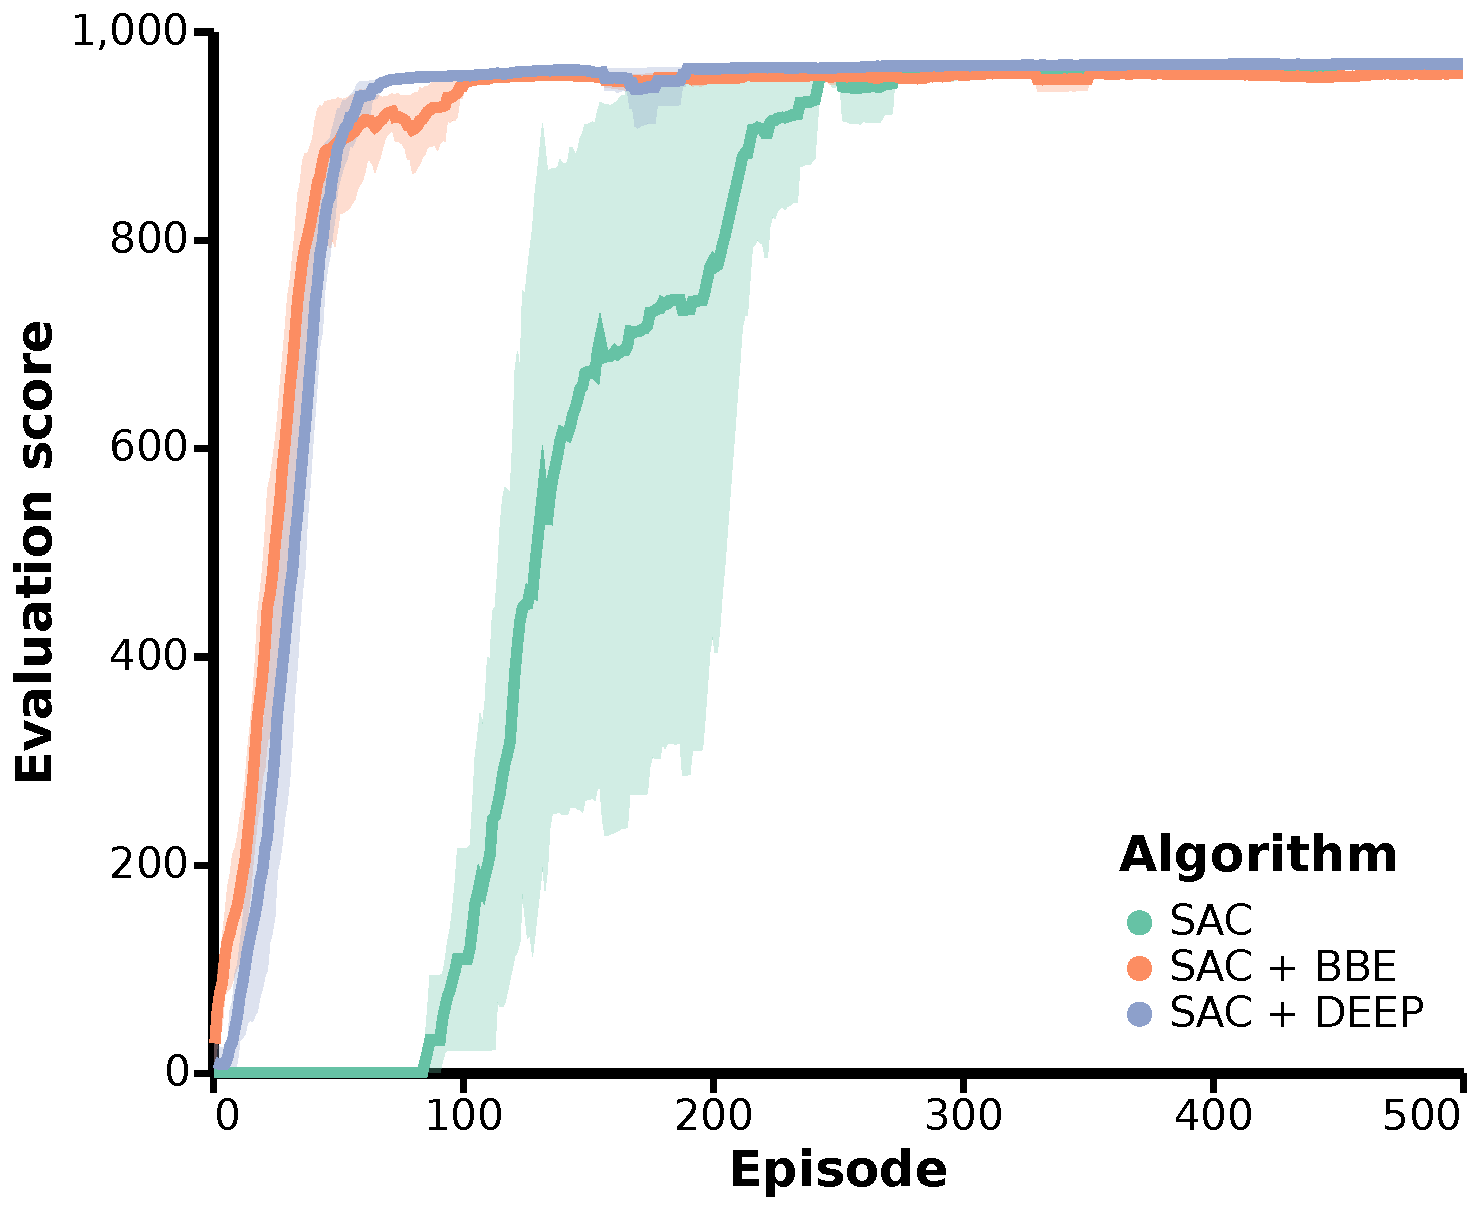
\includegraphics[width=\textwidth]{figures/deep/neurips_ball_in_cup_explore.pdf}
        \caption{Ball-in-cup explore}
    \end{subfigure}
    % \caption{Adding \algshort{} does not result in worse performance on the original ball-in-cup environment. In a version of the environment with resets that do not provide full coverage, \algshort{} performs just as well, whereas the performance of plain SAC is greatly impaired.}
    % \label{fig:ball_in_cup}
    \hfill
    \begin{subfigure}[b]{0.24\textwidth}
        \centering
        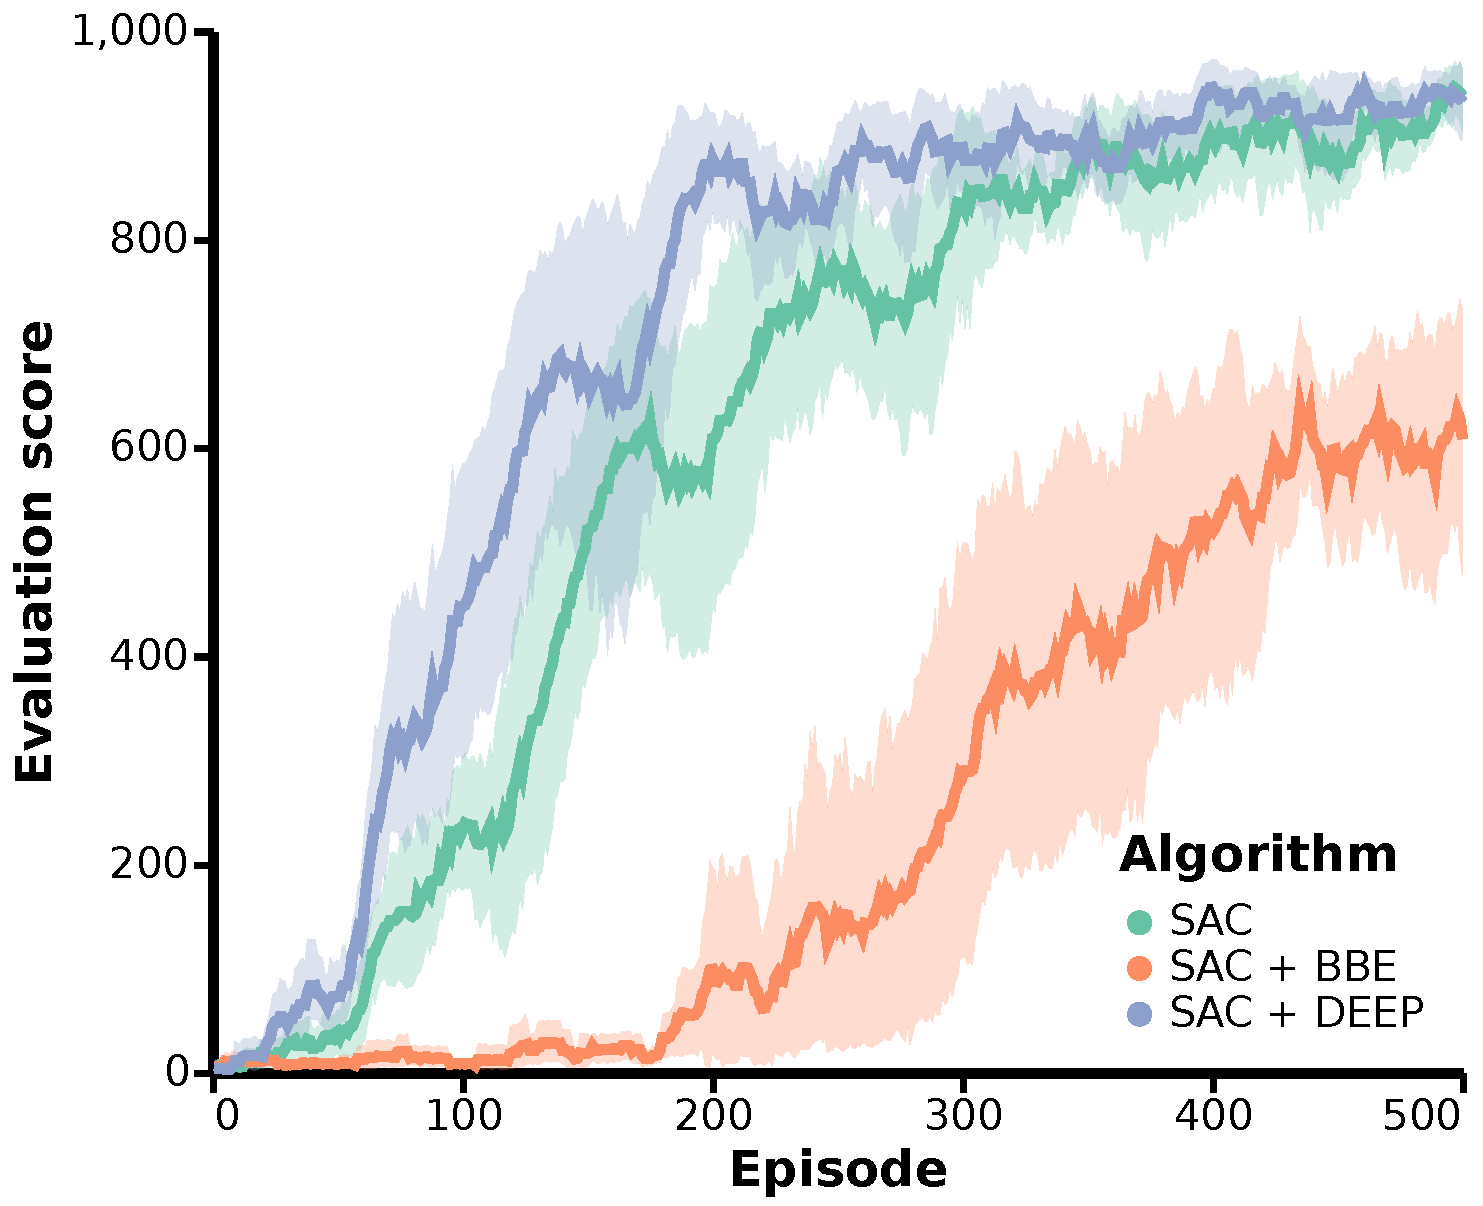
\includegraphics[width=\textwidth]{figures/deep/neurips_reacher.pdf}
        \caption{Reacher}
    \end{subfigure}
    \begin{subfigure}[b]{0.24\textwidth}
        \centering
        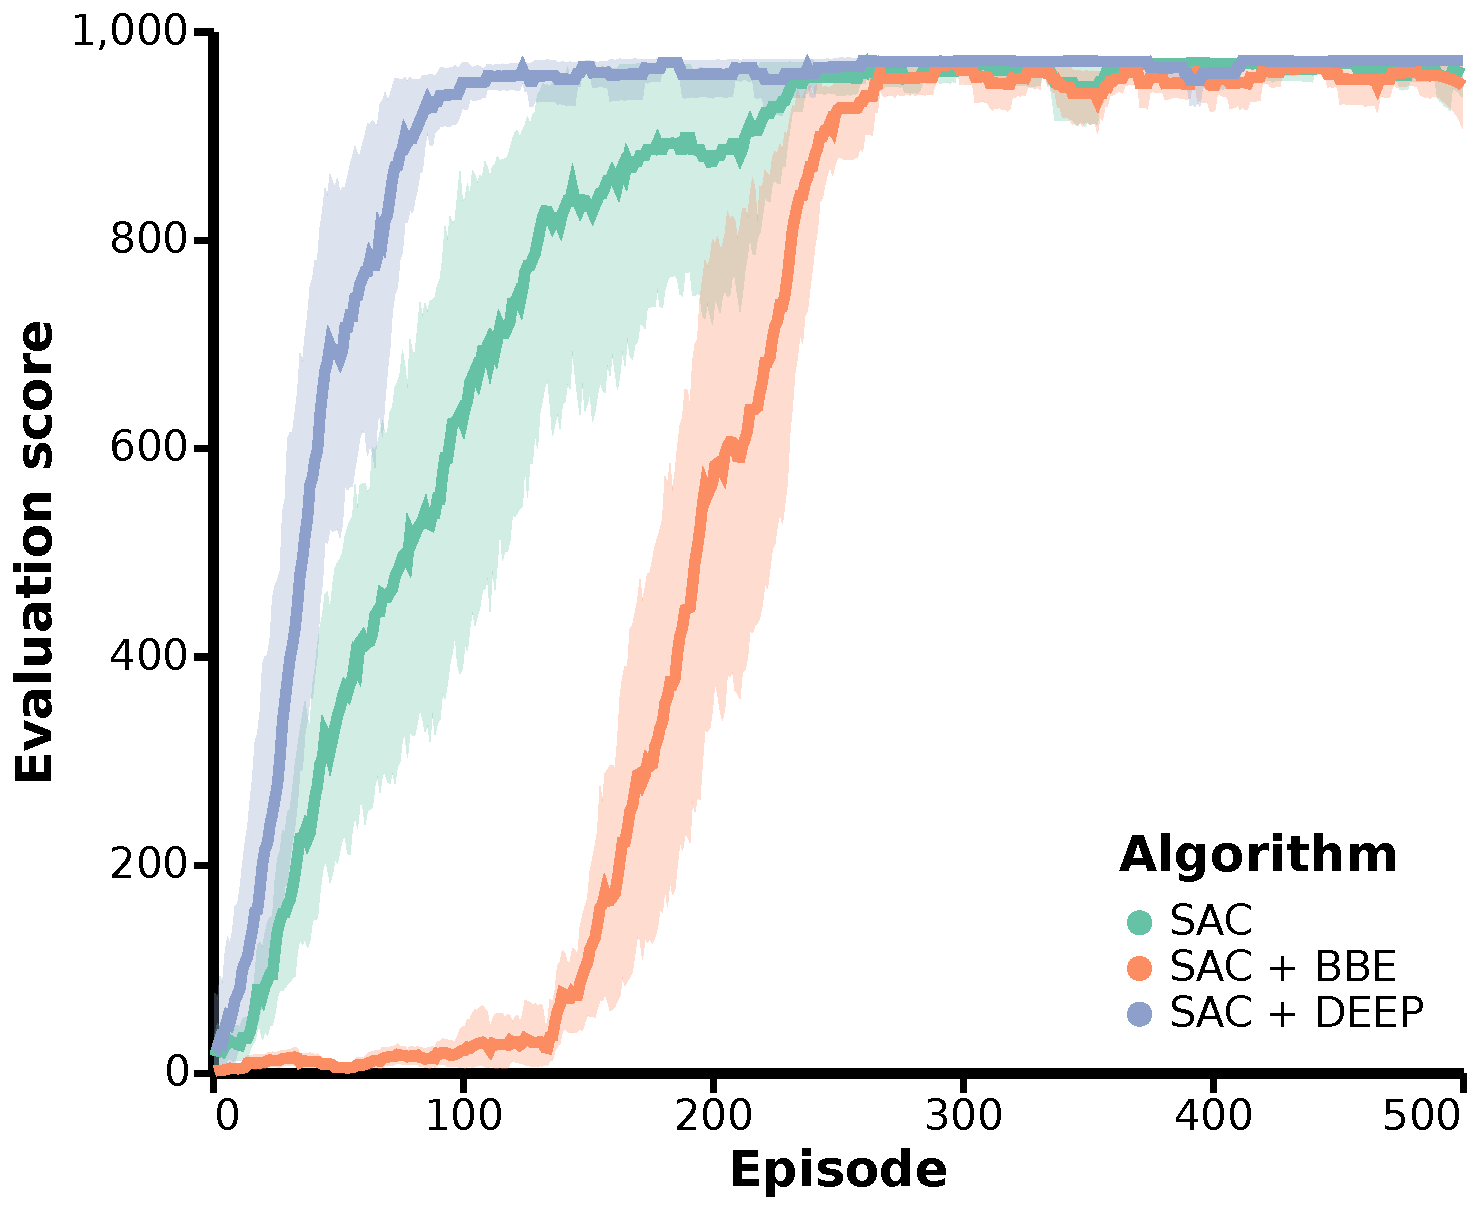
\includegraphics[width=\textwidth]{figures/deep/neurips_reacher_explore.pdf}
        \caption{Reacher explore}
    \end{subfigure}
    % \caption{Results on the original Reacher environment and on a version modified to reset the arm in one quadrant and the target in the opposite quadrant.}
    % \label{fig:reacher}
    \vspace{1em}

    \begin{subfigure}[b]{0.24\textwidth}
        \centering
        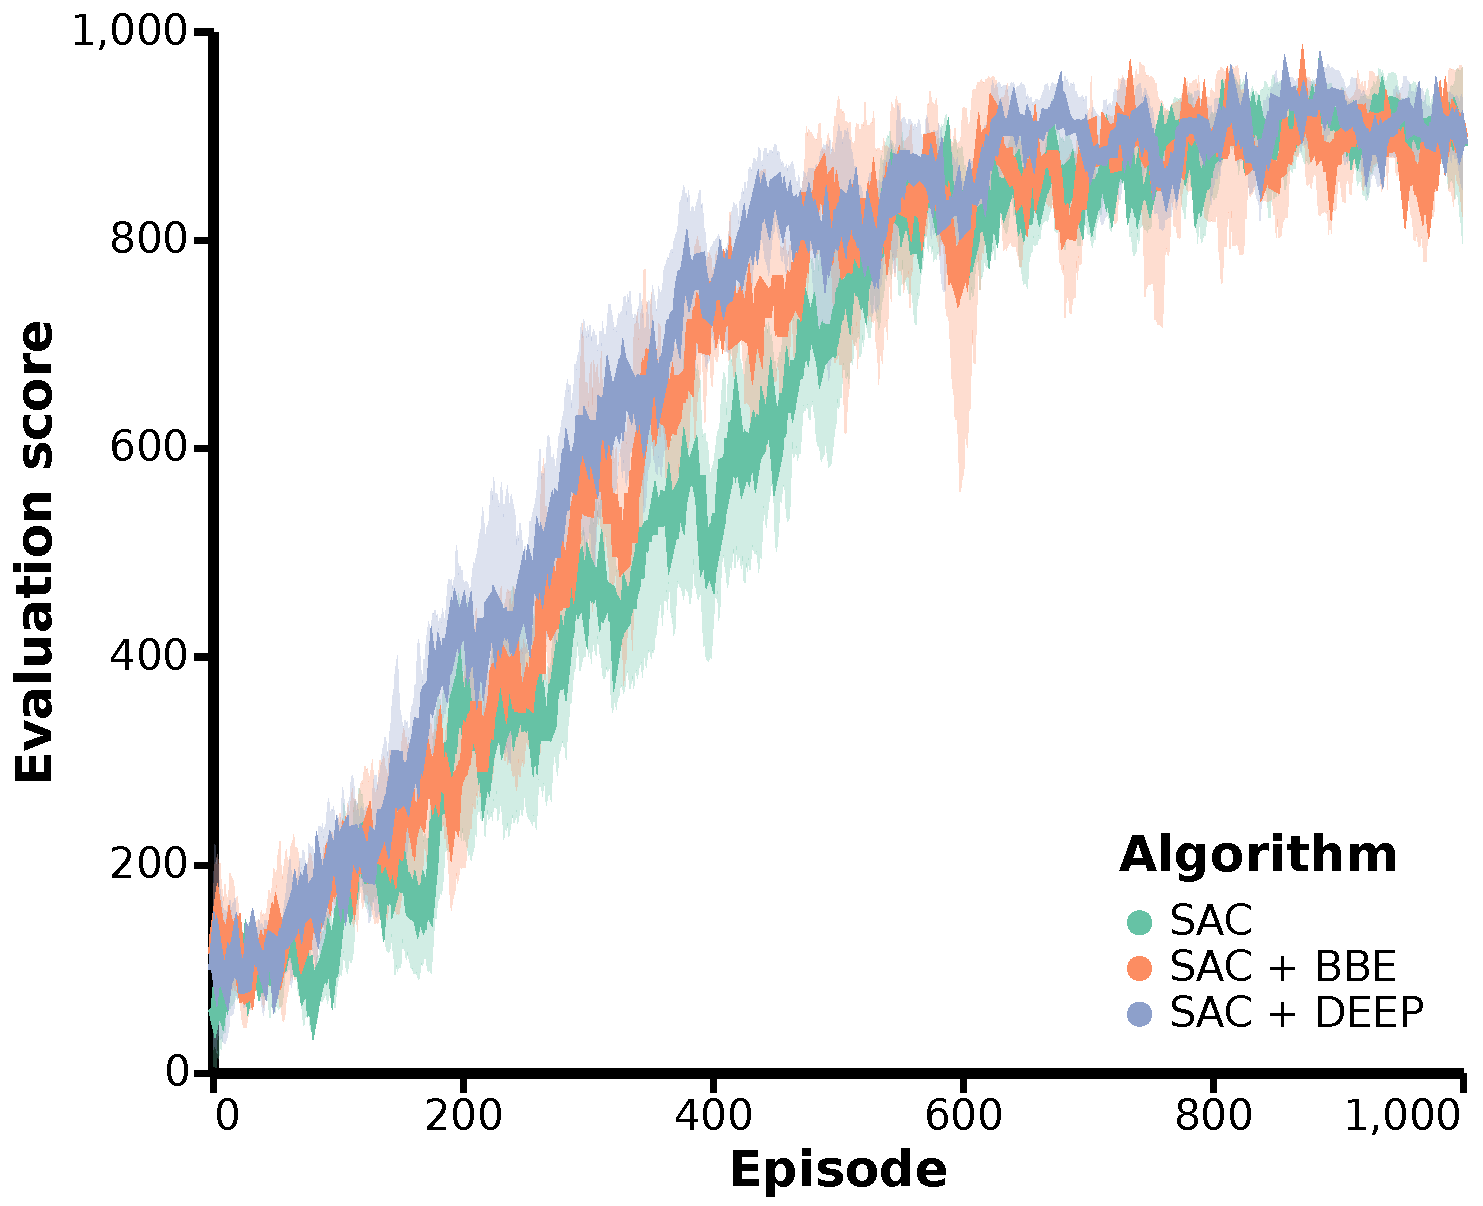
\includegraphics[width=\textwidth]{figures/deep/neurips_finger.pdf}
        \caption{Finger}
    \end{subfigure}
    \begin{subfigure}[b]{0.24\textwidth}
        \centering
        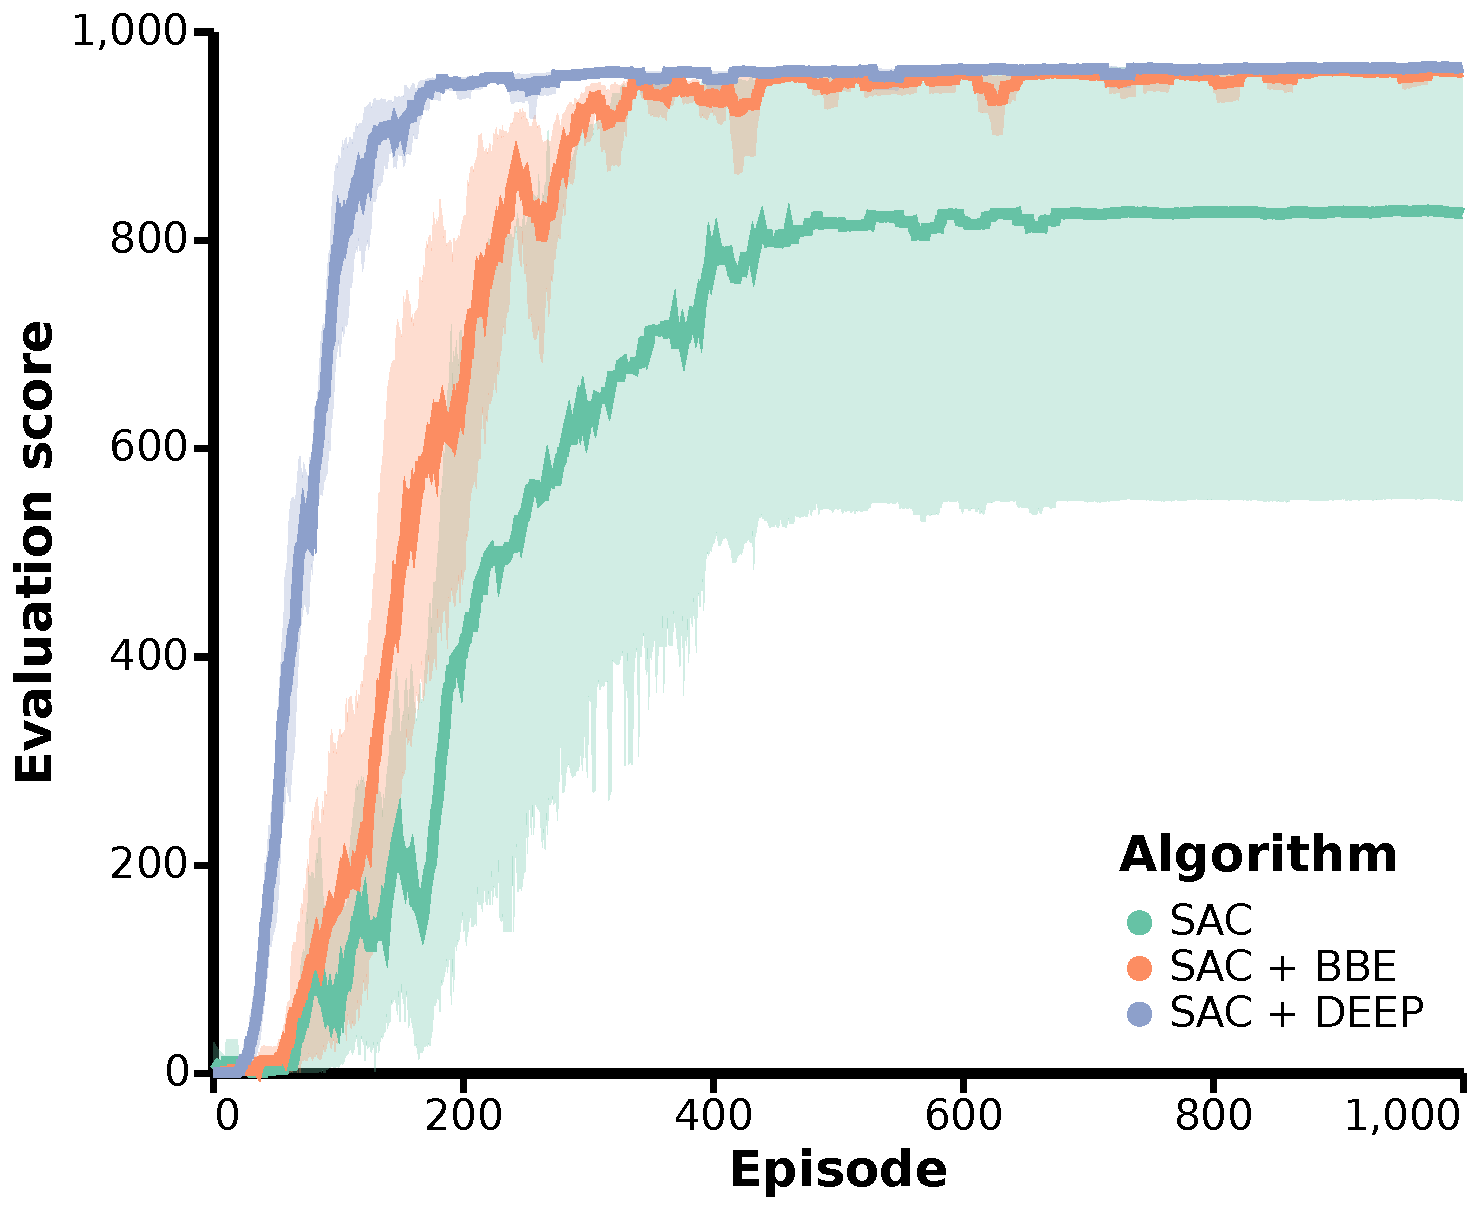
\includegraphics[width=\textwidth]{figures/deep/neurips_finger_explore.pdf}
        \caption{Finger explore}
    \end{subfigure}
    \hfill
    \begin{subfigure}[b]{0.24\textwidth}
        \centering
        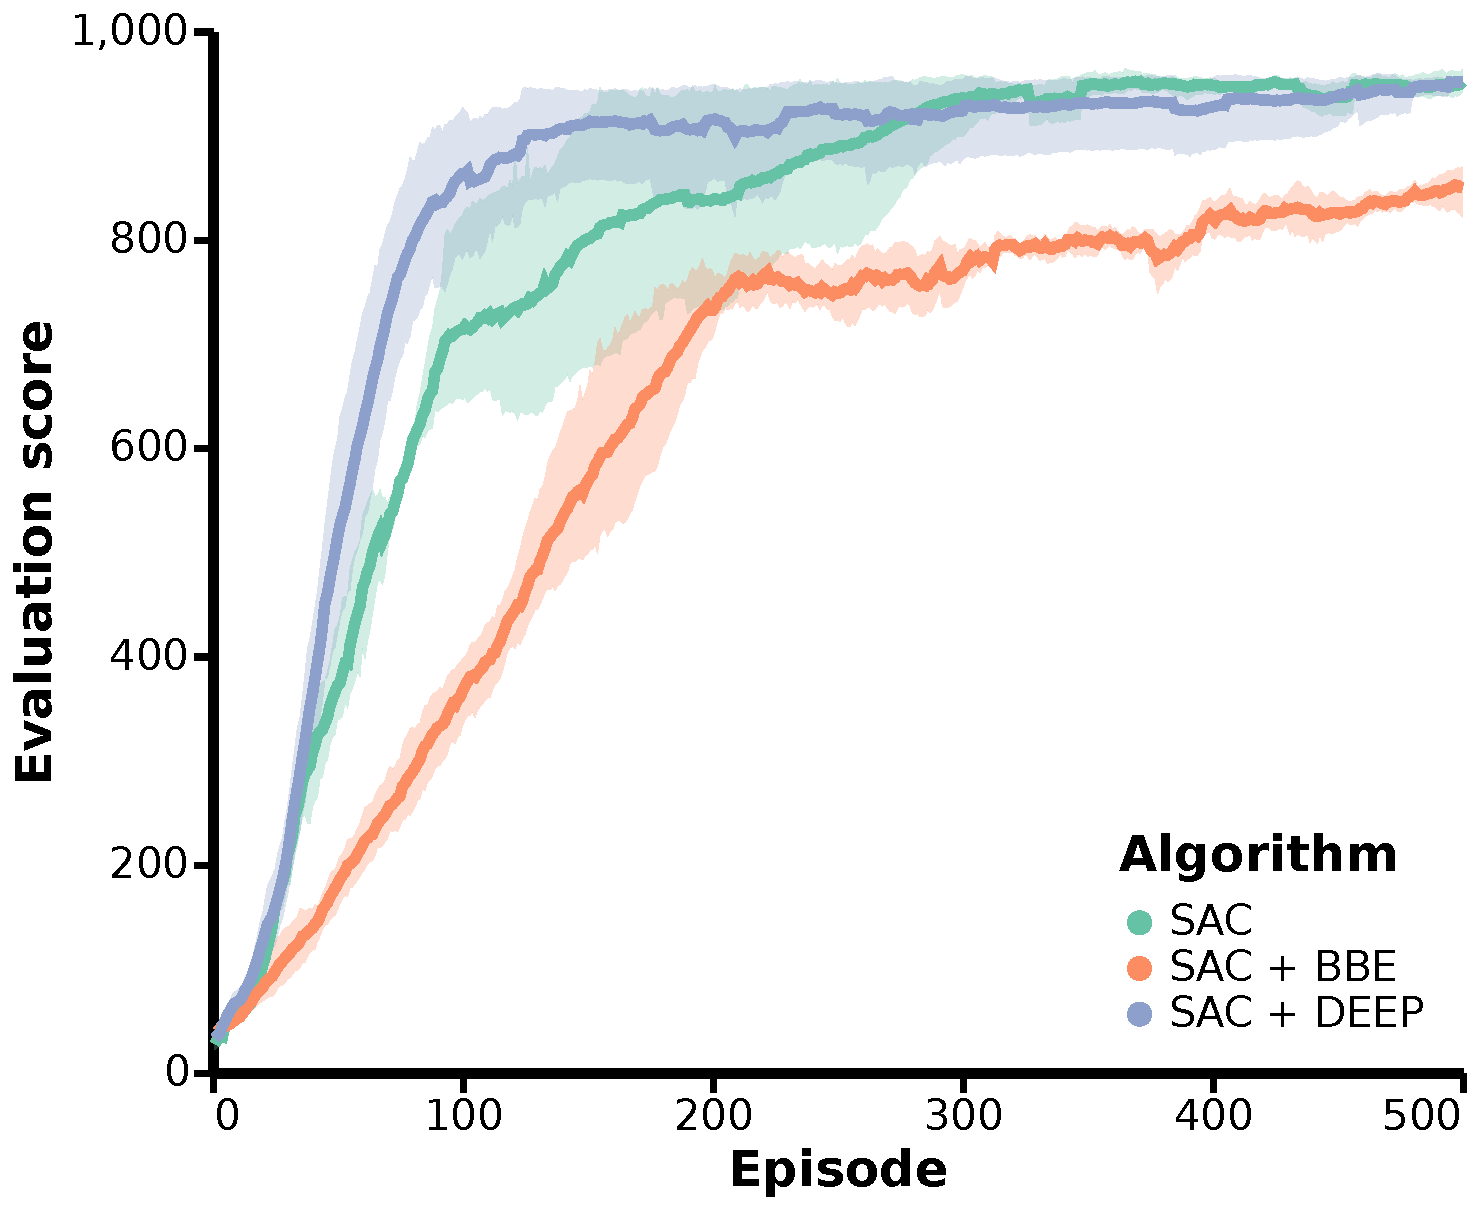
\includegraphics[width=\textwidth]{figures/deep/neurips_walker.pdf}
        \caption{Walker}
    \end{subfigure}
    \begin{subfigure}[b]{0.24\textwidth}
        \centering
        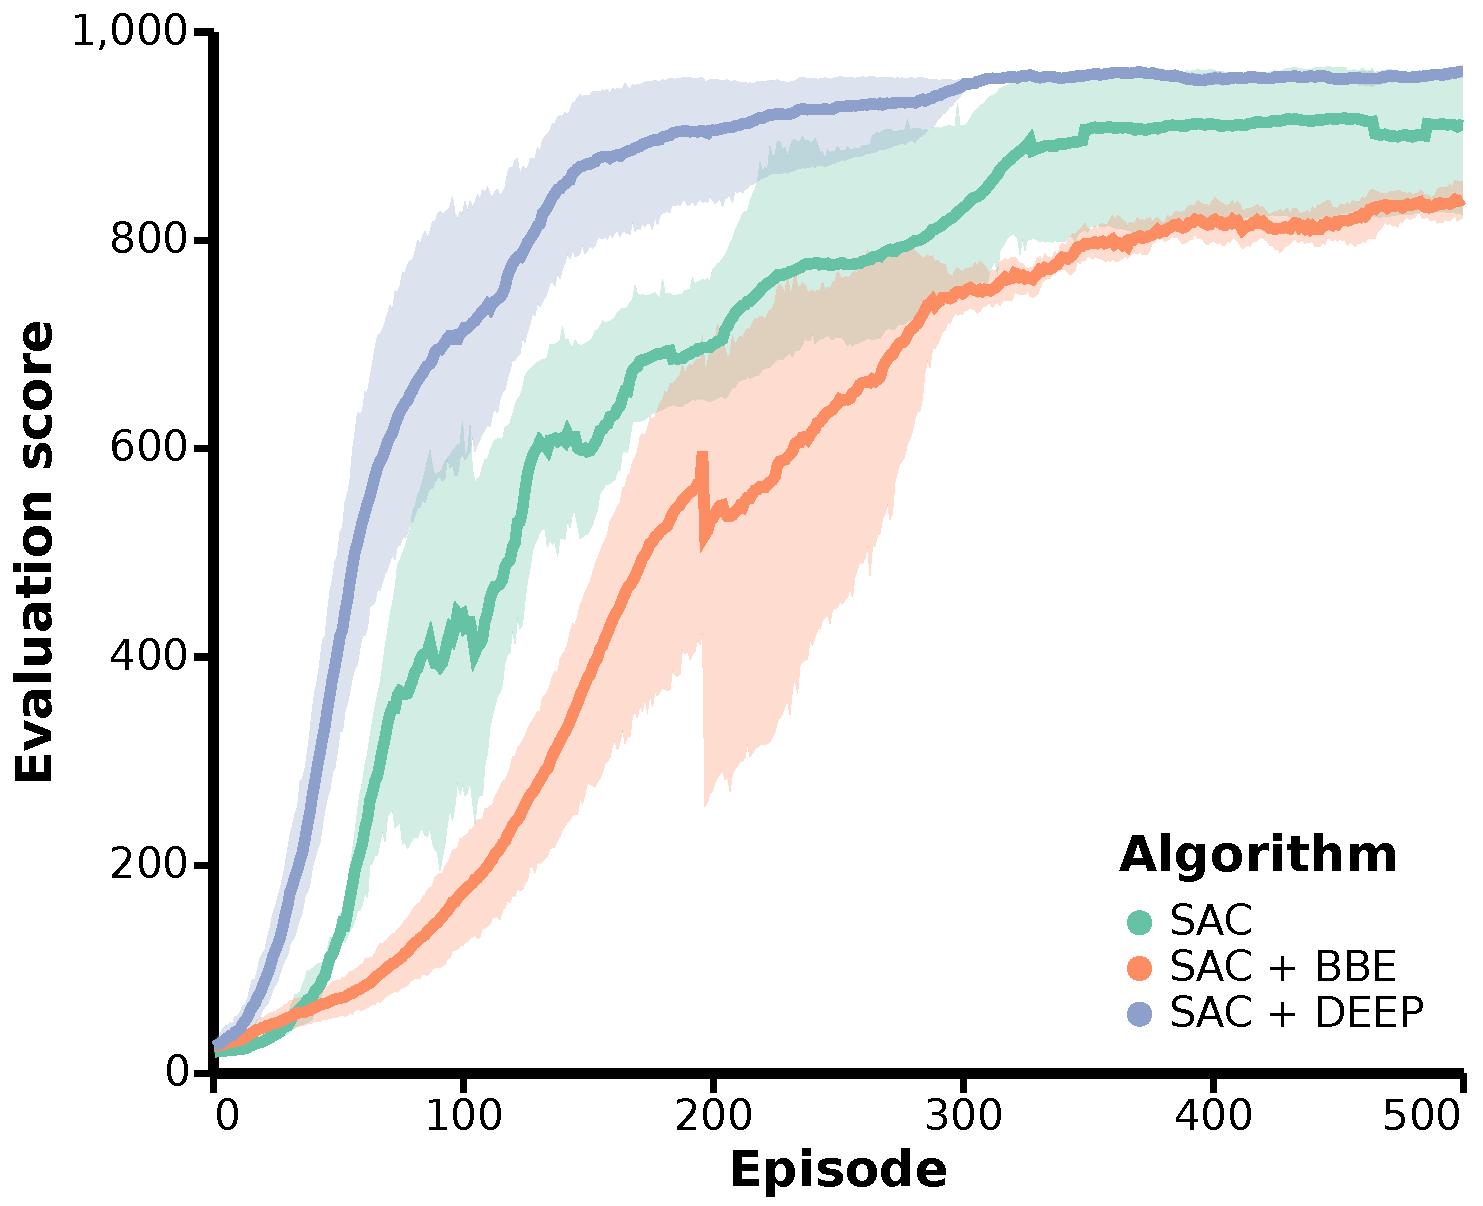
\includegraphics[width=\textwidth]{figures/deep/neurips_walker_explore.pdf}
        \caption{Walker explore}
    \end{subfigure}
    \caption{Results on original Control Suite environments (left in each pair) and modified versions without exploratory resets and rewards (right).
    Across the original environments, SAC + \algshort{} performs as well or better than SAC, while SAC + BBE performs much worse on some environments.
    On the exploration environments, \algshort{} + SAC learns much faster than SAC.
    BBE sometimes provides significant gains over SAC but sometimes performs worse even on exploration environments.
    % \red{(Rename algorithm and make fonts bigger)}}
    }
    \label{fig:control_suite}
\end{figure}

\subsubsection{Environments for evaluating exploration}
% The DeepMind Control Suite \citep{tassa2018deepmind} is a standard benchmark for continuous control RL algorithms.
While Control Suite has driven great progress in policy learning, it was not designed to evaluate an agent's exploration capabilities; in fact, the included environments were selected to be solvable by algorithms with only undirected exploration. From that work:
\begin{quote}
    We ran variety of learning agents (e.g. Lillicrap et al. 2015; Mnih et al. 2016) against all tasks, and iterated on each task’s design until we were satisfied that
    [\ldots]
    % we were satisfied that the physics was stable and non-exploitable, and that
    the task is solved correctly by at least one agent. \citep{tassa2018deepmind}
\end{quote}
Control Suite avoids the need for directed exploration via two mechanisms.
First, in many environments the start state distribution is sufficiently wide (e.g. uniform over reachable states) to guarantee that any policy will see high-value states.\endnote{Some environments, such as Manipulator, additionally start a fraction of episodes at the goal state.}
Second, some environments have rewards shaped to guide the agent towards better performance (e.g. a linearly increasing reward for forward walking speed).

To construct a benchmark for continuous control with exploration, we selected four environments with different objectives (manipulation and locomotion, single-objective or goal-conditional) and observation dimensions (6-24).
We then created ``exploration'' versions of these environments with restricted start state distributions and sparse rewards.
The original environments and their exploration versions together form a benchmark which measures an algorithm's exploration ability and policy convergence.
Environment details are in Appendix \ref{sec:environments_appendix} and their implementation is in the supplement.

\subsubsection{Algorithms}
We include experiments on these eight benchmark tasks with three algorithms: SAC \citep{haarnoja2018softapp} with no additional exploration; BBE with SAC for the policy learner; and \algshort{} with SAC for $\pitask$ and DDQN for $\piexplore$.
BBE and \algshort{} use the pseudo-count reward described in \Cref{sec:kernel_counts} and the SAC implementation is that of \citet{pytorch_sac} with no hyperparameter changes.

The kernel-based exploration bonus used for BBE and \algshort{} requires a scaling law to set the kernel variance as a function of the observation dimension.
We adapt the scaling relationship from \citep{Henderson2012NormalRB} (see Appendix \ref{sec:count_implementation}).
BBE has an additional hyperparameter for the scale of the bonus.
We performed a sweep with values in $\{ 10^{-2}, 10^{-1}, 1, 10 \}$ and found that $1$ performed best overall.
This setting, which makes the maximum bonus equal to the maximum environment reward, ensures that visiting a new state remains the best option until the true goal state is discovered.
Further implementation details are available in Appendix \ref{sec:appendix_benchmark_implementation}.
We additionally performed an ablation which, like \algshort{}, learns separate Q functions for the two rewards, but which learns one policy to maximizes the sum of their Q values.
In our experiments (available in Appendix \ref{sec:benchmark_results_appendix}) this ablation never outperforms BBE, so for clarity we exclude it here.
% Those results are available in Appendix \ref{sec:benchmark_results_appendix}.



\begin{figure}[ht]
    \centering
    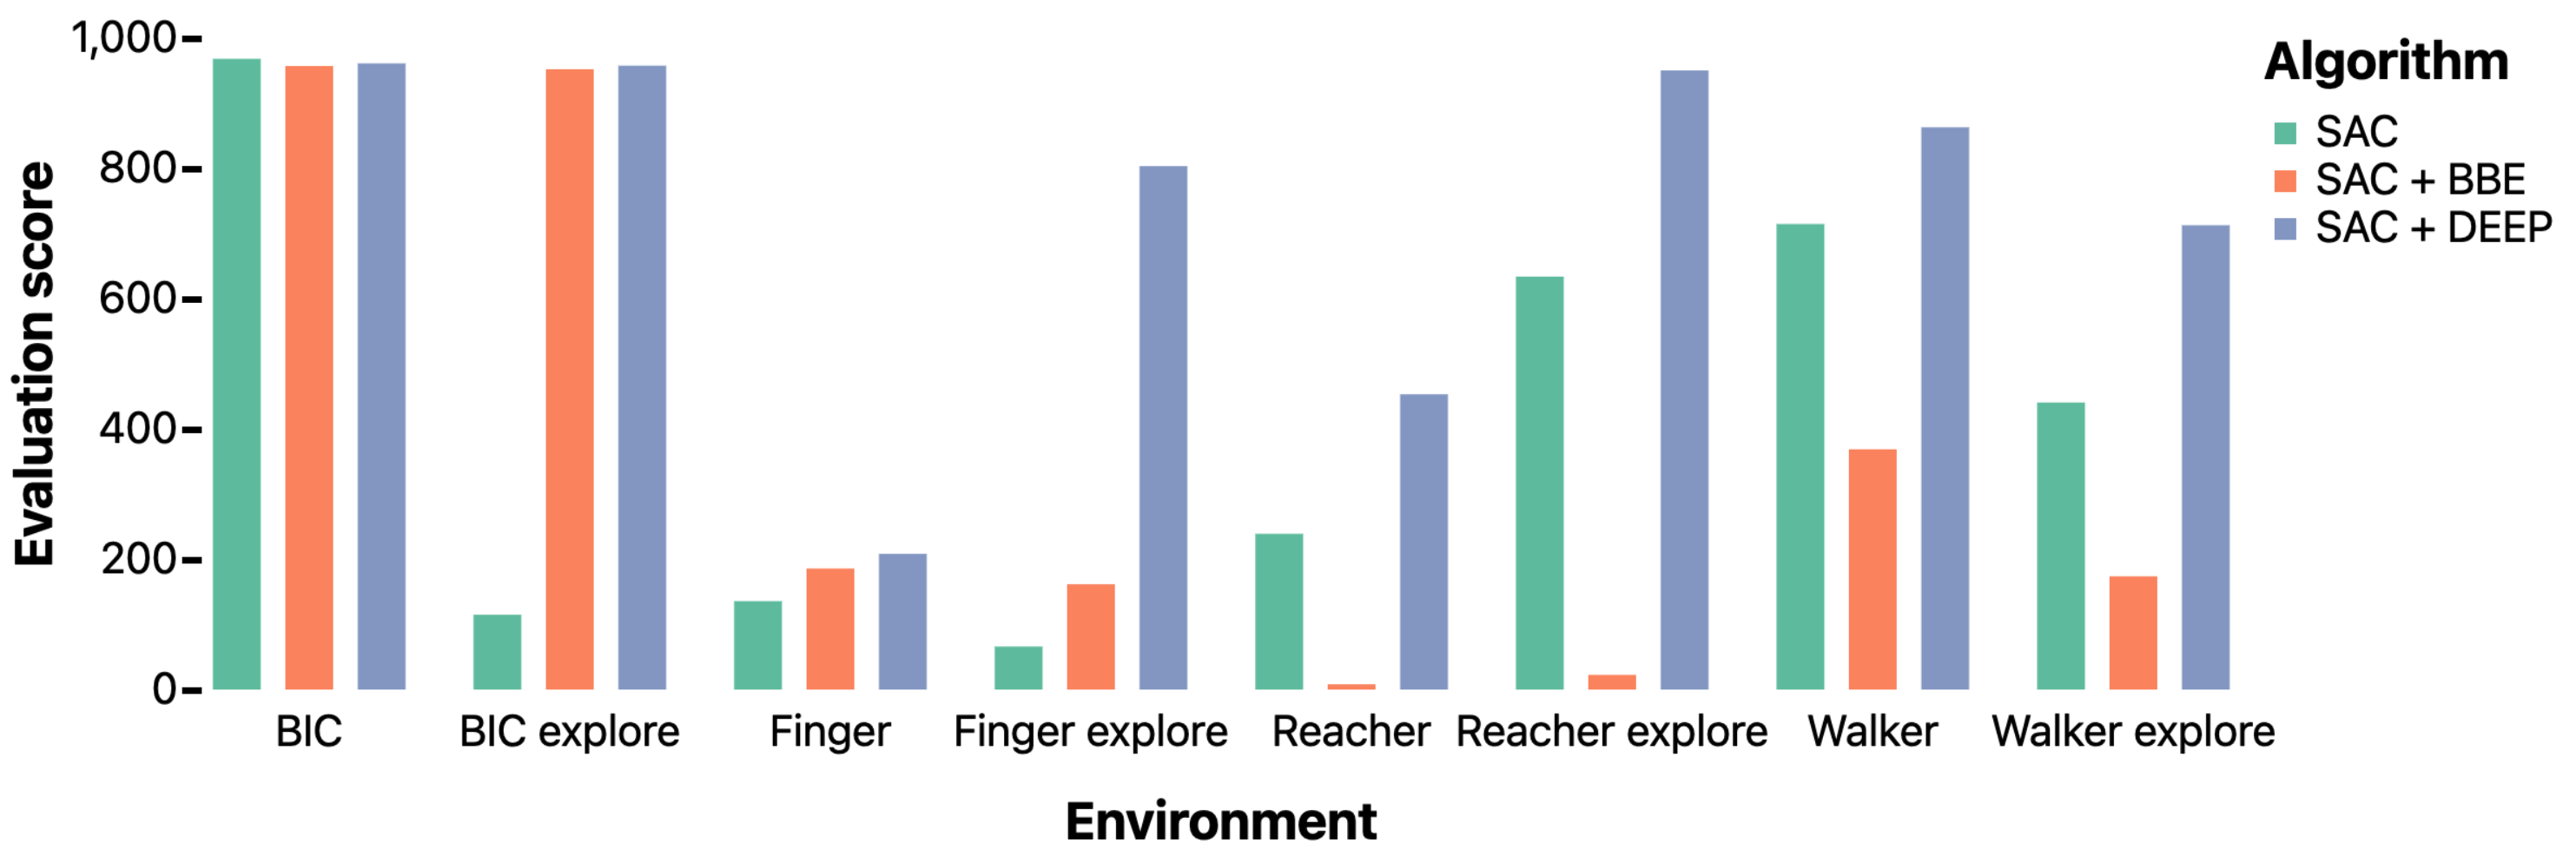
\includegraphics[width=0.95\textwidth]{figures/deep/control_suite_summary_100.png}
    \caption{Results after 100 episodes. In this extremely sample-limited regime, exploration speed and fast policy convergence are both essential. In every environment, SAC with \algshort{} (blue, right column in each set of three) performs comparably to or better than SAC alone or SAC with BBE.}
    \label{fig:control_suite_summary}
\end{figure}

We present experiments on the original versions of four Control Suite tasks and their exploration counterparts.
The results are shown in \Cref{fig:control_suite} with the means and 95\% confidence intervals over 8 seeds.
We find that across the original environments, \algshort{} gives similar or slightly better performance to SAC, while BBE significantly impairs SAC on two of the four environments and matches SAC on the other two.
Across the exploration environments, \algshort{} gives the best performance and sample efficiency.
BBE performs better than SAC alone on two exploration environments and worse than SAC on the other two.
\Cref{fig:control_suite_summary} shows the performance of each algorithm after only 100 episodes, highlighting the substantial benefits from using \algshort{} in the few-sample regime.



Overall, SAC + \algshort{} never performs worse than SAC alone, while yielding substantial improvements in environments where rewarding states are harder to discover.
BBE's more mixed performance provides a possible explanation for the limited influence that methods of that family have had on sample-efficient continuous control, and perhaps more generally on sample-efficient RL.
Given that in this setting the addition of BBE is as likely to harm as to help, its lack of adoption is unsurprising.








\section{Related work}

\paragraph{Sample-efficient continuous control.}
% As discussed in the introduction, there has been a large amount of progress on sample efficient off-policy RL that
Our method leverages progress on sample efficient off-policy RL, as it can be combined with any off-policy algorithm.
A strong line of work has brought the sample complexity of model-free control within range of solving tasks on real robots \citep{Popov2017DataefficientDR,kalashnikov2018qt,haarnoja2018soft,fujimoto2018addressing,haarnoja2018softapp,Abdolmaleki2018MaximumAP}.

% In general, current RL algorithms can be clustered into two categories: on-policy algorithms which are reliable but require hundreds of millions of environment steps to solve tasks \citep{Mnih2016AsynchronousMF,Schulman2015TrustRP,schulman2017proximal}, and recent off-policy algorithms which have brought the sample complexity of model-free control within range of solving tasks on real robots \citep{Popov2017DataefficientDR,kalashnikov2018qt,haarnoja2018softA,fujimoto2018addressing,haarnoja2018softapp,Abdolmaleki2018MaximumAP}.

%\subsection{Exploration in deep RL}

\paragraph{Bonus-based exploration.}
There have been many bonuses proposed in the BBE framework.
Several works \citep{Stadie2015IncentivizingEI,pathak2017curiosity,burda2018exploration} propose to use prediction error of a learned model to measure a transition's novelty, with the key differences being the state representation used for making predictions.
% \citet{Stadie2015IncentivizingEI} make predictions in the raw observation space, while \citet{pathak2017curiosity} use a learned embedding from an inverse dynamics model, and \citet{burda2018exploration} use a randomly-initialized neural network to embed the states.
\citet{houthooft2016vime} propose a bonus based on the information gain of the policy.
\citet{bellemare2016unifying} and others \citep{ostrovski2017count,Tang2017Exploration} use continuous count analogues to calculate the count-based bonuses of \citet{strehl2008analysis}.
%  also use the bonus formula from \citet{strehl2008analysis}, but compute counts using a locality-sensitive hashing function to bin the states.
\citet{Machado2020CountBasedEW} use the norm of learned successor features as a bonus, and show that it implicitly counts visits.
Unlike previous work, our paper focuses on the updates and representation of the behavior policy, and \algshort{} can be used in conjunction with any of these bonuses.
Never Give Up \citep{Badia2020NeverGU} uses an episodic exploration bonus and trains policies with different bonus scales including a task policy.
% exploration bonus with an episodic structure, encouraging a behavior policy to visit each state infinitely often while rapidly adapting the reward within each episode.
% Instead of a single policy, NGU learns an ensemble of policies with different scales of the exploration bonus, allowing it to act greedily with respect to a task policy.
However, it is designed to maximize asymptotic performance rather than sample efficiency and does not learn faster than a baseline early in training.


\paragraph{Optimism.}
Classic exploration methods \citep{Kearns1998NearOptimalRL,Brafman2002RMAXA,strehl2008analysis,Jaksch2008NearoptimalRB}, depend on an optimistically-defined model.
Model-free methods with theoretical guarantees \citep{Strehl2006PACMR,Jin2018IsQP} use Q functions initialized optimistically.
% Optimism is difficult to ensure with neural networks, since even an optimistic initialization will rapidly wash out due to generalization from other observed points.
Similar to our \cref{eq:optimism}, \citet{Rashid2020OptimisticEE} propose a method for ensuring optimism in Q learning with function approximation by using a count function.
% Our method uses a similar formulation for learning an optimistic exploration Q function.
However, \algshort{} leaves the task policy unbiased in the few-sample regime by separating the exploration policy from the task policy.


\paragraph{Temporally-extended actions.}
A variety of work proposes to speed up $\epsilon$-greedy exploration via temporally-extended actions which reduce dithering.
Some methods \citep{Schoknecht2003ReinforcementLO,neunert2020continuousdiscrete} propose to bias policies towards repeating primitive actions, resulting in faster exploration without limiting expressivity.
\citet{Dabney2020TemporallyExtendedE} describe a temporally-extended version of $\epsilon$-greedy exploration which samples a random action and a random \emph{duration} for that action.
\citet{Whitney2020Dynamics-Aware} use a learned temporally-extended action space representing the reachable states within a fixed number of steps.
While these methods improve over single-step $\epsilon$-greedy, they are unable to perform directed exploration or discover faraway states.


\paragraph{Randomized value functions.}
Modern works \citep{Osband2016DeepEV,osband2019deep} extend Thompson sampling \citep{thompson1933likelihood} to neural networks and the full RL setting.
Relatedly, \citep{Fortunato2018NoisyNF,Plappert2018ParameterSN} learn noisy parameters and sample policies from them for exploration.


\section{Discussion}
In this paper we have investigated the potential for directed exploration to improve the sample efficiency of RL in continuous control.
We found that BBE suffers from bias and slow state coverage, leading to performance which is often worse than undirected exploration.
We introduced \algname{}, which separately learns an unbiased task policy and an exploration policy and combines them to select actions at training time.
\algshort{} pays no performance penalty even on dense-reward tasks and explores faster than BBE.
In our experiments, \algshort{} combined with SAC provides strictly better performance and sample efficiency than SAC alone.
We believe that with its combination of reliable and efficient policy learning across dense and sparse environments, SAC + \algshort{} provides a compelling default algorithm for practitioners.

% \clearpage
\printendnotes
